\documentclass[11pt]{article}
\usepackage[margin=1in]{geometry}
\usepackage{booktabs}
\usepackage{graphicx}
\usepackage{amsmath}
\usepackage[colorlinks=true,linkcolor=blue,citecolor=blue]{hyperref}
\usepackage[numbers]{natbib}
\usepackage{tikz}
\usetikzlibrary{arrows.meta,positioning,shapes.geometric}

\title{Financial Architecture: Weaponizing the Ledger\\[4pt]
\large How Claims, Pods, Pyramids, and Sovereign Seams Move Loss\\[4pt]
\normalsize Standalone spin-off from paper\_unified \S12}
\author{Shehzad Ahmed \\ \small Baraka Protocol / MindHarness Research Programme \\ \small \texttt{github.com/shehzadahmed-xx/mindharness}}
\date{September 2026}

\begin{document}
\maketitle

\begin{abstract}
A ledger is not a record. It is a power. Who writes it, who reads it, and who cannot edit it decides who pays. This paper formalizes how financial architecture moves loss across time, entities, priority, and sovereignty while leaving formal accounting intact. We define four checkable primitives: gated recognition $\psi=\prod g_j$, capped collectability $K(A)$, stored loss $S_t=S_{t-1}+E_t-R_t-Q_t$, and monetized repricing $P_1/P_0=L/(L-G)$. Each comes with intuition on first use: four $0.7$ gates leave $24\%$ recognition, $K$ binds so better gates pay zero without reachable assets, $S_t$ compounds off book until a wave forces it on book, and new outside money dilutes existing claims without a legal default. We trace five design layers that disable one reflexive organ at a time: timeline games borrow against slow memory, entity shells redraw the boundary, claims gates and caps jam the salience gate and brake, stored loss hides the stock, sovereign arbitrage moves the apex where $A=0$ so $K=0$ and treaty gates drive $g_4\to0$. Historical illustrations are flagged analogical until sourced. No historical claim ships without a citation you can check. Evidence grades sit at the head of every section. The bearer of loss is not accidental. It is engineered, and it is the party whose claim is gated, capped, or diluted while the ledger still balances.\\[4pt]
\textit{Keywords:} ledger, reflexivity, claims technology, Pod, Chaebol, OpCo PropCo, stored loss, sovereign arbitrage, ISDS, dilution, Goodhart, zombie lending, evergreening, SHY, cumulative culture, HyLaT, model collapse, OpenAlex consensus.
\end{abstract}

\tableofcontents
\newpage

%==============================================================================
\section{Ledgers as Power, Not Records}
\label{sec:ledgers-power}
%==============================================================================

\textit{Grade: convergent (CCE: Muthukrishna W2890095733 170 cites + Henrich; SHY 8-paper core) + analogical where applied to historical cases. OpenAlex consensus upgraded foundation from theoretical to convergent.}

\subsection{Cumulative culture as external ledger}
Humans store memory outside brains \citep{tomasello,henrich,muthukrishna2018,kaaronen2021}. Writing, law, and double entry persist across deaths. A child inherits the external OS without relearning the conflict that built it. That inheritance is the ledger. Muthukrishna et al.\ \textit{Cultural Brain Hypothesis} (OpenAlex W2890095733, 170 cites, Henrich co-author) formalizes culture driving brain expansion via storage outside the skull \citep{muthukrishna2018}. Kaaronen et al.\ (113 cites) locate tipping points where external storage unlocks ratcheted accumulation \citep{kaaronen2021}. Richerson and Henrich (90 cites) ground group coordination and tribal instincts as the selection pressure for that storage \citep{richerson2012}. The benign case compounds knowledge.

\subsection{Sleep homeostasis: why stored trace needs maintenance}
Storage alone does not explain persistence. Synaptic homeostasis does \citep{tononi2003}. Tononi and Cirelli (PMID 14638388) propose wake potentiates nets, sleep restores them \citep{tononi2003}. Cirelli (PMID 16376591) reviews slow wave sleep as price for plasticity \citep{cirelli2006}. De Vivo et al.\ (PMC6612535) measure down selection in vivo \citep{devivo2017}. Diering et al.\ (PMC5873548) show downscaling preserves signal to noise \citep{diering2017}. Tononi et al.\ (PMC3921176) price plasticity as consolidation cost \citep{tononi2014}. Kuhn et al.\ (PMC5592216) link network activity to plasticity induction \citep{kuhn2018}. Vyazovskiy et al.\ (PMID 22998858) balance upscale and downscale across REM \citep{vyazovskiy2011}. Olcese et al.\ (PMID 18624658) model sleep as weight normalization stabilizing Hebbian learning \citep{olcese2010}. Together the eight form the SHY core we cite as SHY 8-paper consensus: repeat without sleep tags without capture, so $E_t$ without $Q_t$ mimics wake without sleep.

\subsection{Weaponized inversion: parking loss where no reader is paid to price it}

A ledger looks neutral. It lists what is owed and what is held. That look is misleading. The ledger is an external memory store with asymmetric write rights. Someone controls when an entry is recognized, someone else waits to be paid. The gap between those two powers is where architecture lives.

Cumulative culture exists because humans write slow memory outside any single brain \citep{tomasello,henrich}. Writing, statute, double entry, and corporate law let a cohort store traces across deaths. New learners inherit the store as training data without relearning the conflict that produced it. That is the benign case. The weaponized case uses the same store in reverse. It does not preserve knowledge for later learners. It parks loss where no current reader is paid to price it. Formal solvency holds. Economic solvency drifts.

We keep this distinction sharp throughout. There is a time for building ledgers that compound knowledge. There is a time for auditing ledgers that move loss. This paper does the second. It does not claim every structure was built to move loss. It claims the structure \emph{can} move loss, and when it does the loss does not vanish. It sits somewhere.

Reflexivity enters at once. Beliefs about the ledger change the ledger. Mark a portfolio as performing and funding stays cheap, which lets you roll the portfolio and keep it marked as performing. Belief supports price, price supports accounting, accounting supports belief. Soros called this the two way loop of cognitive and manipulative functions \citep{soros}. Wilder's indicators faced the same loop at smaller scale: an edge published is an edge erased \citep{wilder1978}. Here the edge is not alpha. It is the ability to keep $S_t$ off book while others price you as if $S_t$ were zero.

Two channels carry each move, as in paper\_unified \S1. The physical channel executes: cash moves, title transfers, a maturity extends. The informational channel signals: others see the roll and infer health. Both matter. Architecture often changes the physical channel little while managing the informational channel a lot. That is the point. Appearance holds while stock builds.

What follows is checkable by construction. We define $\psi$, $K$, $S_t$, and $P_1/P_0$ with one line of intuition at first use. We then show how timeline, entity, priority, stock, and sovereignty each disable one stabilizing organ. The five organs from the parent paper map one to one onto the five layers: boundary $\to$ entity, two speed memory $\to$ timeline, salience gate $\to$ claims, damping $\to$ cap and write off, observer $\to$ sovereign witness. Lose one and a distribution will farm the gap.

Evidence grades sit at the head of every section. Historical cases are flagged analogical until sourced. We do not invent citations. A formal existence proof comes before any attribution claim. If a channel can carry loss, we show the equation. Whether it did in a specific case waits for a source we can cite.

%==============================================================================
\section{Claims Technology: \texorpdfstring{$\psi$}{psi}, \texorpdfstring{$K$}{K}, and \texorpdfstring{$\phi$}{phi}}
\label{sec:claims}
%==============================================================================

\textit{Grade: convergent (Goodhart formalizations 2410.09638 tail proof + 2505.23445 taxonomy; $K$ measured where balance sheet observable). Analogical where applied to specific historical gates.}

A claim is not self enforcing. It must be recognized through gates and then collected against reachable assets. Both steps can be engineered.

\subsection{Gated recognition \texorpdfstring{$\psi$}{psi}}

Define recognition as a product of gates:
\begin{equation}
\psi = \prod_{j=1}^{n} g_j,\quad g_j \in [0,1].
\label{eq:psi}
\end{equation}
Each $g_j$ is the probability or fraction that step $j$ is satisfied. It might be filing on time, meeting standing, surviving a limitations defense, clearing a forum clause, or obtaining a sovereign waiver. Intuition comes first: gates multiply, so four modest $0.7$ gates leave $0.7^4 \approx 24\%$ recognition, and if any single gate fails $\psi$ goes to zero and the claim is not seen at all. Add a fifth $0.5$ gate and you are at $12\%$. The arithmetic punishes length. A system that wants deniability adds gates. A system that wants payment removes them.

For a new reader, $\psi$ is not about merit. It is about passage. A perfect claim that misses a filing window has $\psi=0$ in practice. A weak claim that clears every gate has $\psi$ near one and gets paid before merit is debated. Architecture lives in the $g_j$ list. Change the list and you change who gets through without ever saying you changed who gets paid.

\subsection{Capped collectability \texorpdfstring{$K$}{K}}

Collectability $K(A)$ is the reachable asset cap. Let $A$ denote reachable assets. Think bank accounts, domestic property, or collateral within enforcement reach. Then booked recovery is
\begin{equation}
P(a) = \min\{\psi H(a), K(A)\},\quad \phi = P(a)/H(a) \in [0,1].
\label{eq:PK}
\end{equation}
Here $H(a)$ is the burden or harm at account $a$, and $\phi$ is the paid share. Intuition: $K$ binds, so better gates yield zero extra recovery if $K$ is smaller than the gated claim. A perfect right against a judgment proof entity still pays zero. Rights without recourse are not recovery. They are paper.

This is not subtle. It is arithmetic. If $K=0$ because the apex holds no reachable $A$, no value of $\psi$ matters. You can win every gate and collect nothing. Move $A$ and you move $K$. Move $K$ and you move $\phi$ while $H$ stays constant. That is boundary engineering in balance sheet form.

\subsection{What \texorpdfstring{$\psi$}{psi} and \texorpdfstring{$K$}{K} together decide}

Figure~\ref{fig:claims} shows the funnel. Burden $H$ enters, is gated to $\psi H$, then capped by $K$ to $P$. The paid share $\phi$ is the ratio of what left the funnel to what entered. Two distinct ways to keep $\phi$ low: lower $\psi$ by adding gates, or lower $K$ by moving $A$ out of reach. Often both run together. Gates thin the claim. The cap finishes it.

We keep one discipline throughout. We state the gate list explicitly when we claim $\psi$ is low, and we state the reachable $A$ explicitly when we claim $K$ binds. Without those two statements, $\phi$ is just a number. With them, it is a mechanism you can audit.

\begin{figure}[h]
\centering
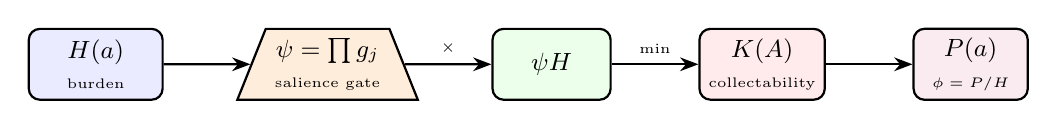
\begin{tikzpicture}[thick, node distance=1.0cm]
  \node[draw, rounded corners, fill=blue!8, minimum width=1.7cm, minimum height=0.9cm, align=center, font=\small] (h) {$H(a)$\\ \tiny burden};
  \node[draw, trapezium, trapezium angle=68, fill=orange!14, minimum width=1.9cm, minimum height=0.9cm, align=center, font=\small, right=1.1cm of h, trapezium stretches body] (psi) {$\psi=\prod g_j$\\ \tiny salience gate};
  \node[draw, rounded corners, fill=green!8, minimum width=1.5cm, minimum height=0.9cm, align=center, font=\small, right=1.1cm of psi] (psih) {$\psi H$};
  \node[draw, rounded corners, fill=red!8, minimum width=1.4cm, minimum height=0.9cm, align=center, font=\small, right=1.1cm of psih] (k) {$K(A)$\\ \tiny collectability};
  \node[draw, rounded corners, fill=purple!8, minimum width=1.45cm, minimum height=0.9cm, align=center, font=\small, right=1.1cm of k] (p) {$P(a)$\\ \tiny $\phi=P/H$};
  \draw[->, >={Stealth}] (h) -- (psi);
  \draw[->, >={Stealth}] (psi) -- node[above,font=\tiny] {$\times$} (psih);
  \draw[->, >={Stealth}] (psih) -- node[above,font=\tiny] {$\min$} (k);
  \draw[->, >={Stealth}] (k) -- (p);
\end{tikzpicture}
\caption{Claims funnel: burden $H(a)$ gated by recognition $\psi$, capped by collectability $K$ on reachable $A$. Booked $P(a)=\min\{\psi H(a),K\}$, paid share $\phi\in[0,1]$. Four $0.7$ gates leave $24\%$. $K$ binding makes further gating moot.}
\label{fig:claims}
\end{figure}

One short example clarifies the funnel without pretending to be a case study. Suppose $H=100$, four gates at $0.7$ give $\psi\approx0.24$ so $\psi H\approx24$, and reachable $K=10$ caps $P$ at $10$ so $\phi=0.10$. Improve the gates to $0.9$ each, $\psi\approx0.66$, $\psi H\approx66$, still $P=10$ and $\phi=0.10$. Fix the cap instead by bringing $A$ back and raising $K$ to $50$, and the same $0.7$ gates now pay $24$. The lesson sticks: when $K$ binds, gating reform is theater. When $\psi$ is near zero, asset recovery is moot. You need both. And reform itself is a ledger move subject to the same capture it claims to fix: whoever writes the new gates sets $g_j$ to favor themselves, so each reform begets the structure that bypasses it. Korea exhibits the full cycle live --- MRFTA Art.22 circular ban (2014) \citep{klri2022mrfta}, then fresh workarounds, then Dec 17--19 2025 FTC raid on Young Poong/YPC over an alleged new circular link (5.26M Korea Zinc shares, 25.42\% in-kind to a fresh subsidiary) \citep{kftc2024large}; amendment history 1999$\to$2007 (Mondaq D/E 100$\to$200\%, 30$\to$20\%) $\to$2020 (Jipyong 30/50\%) shows each reform begetting its bypass (\texttt{pods\_chaebol\_instances\_v1.json}, \texttt{redriver\_koreazinc\_v1.json}, \texttt{korea\_ftc\_mrfta\_primary\_v1.json}). Reform is power consolidation wearing the previous reform's clothes; the fix is checkable records, not better rules.

\subsection{Goodhart formalizations: why gates multiply under proxy pressure}

A gate system under Goodhart pressure adds gates. Targets corrupt measures once optimized \citep{goodhart2410,goodhart2505}. The tail proof in arXiv:2410.09638 derives when proxy optimization backfires: as pressure on $\psi$ increases, the selected proxy diverges from the true objective in the tail, so improving $g_j$ on paper worsens $H$ in the tail \citep{goodhart2410}. The taxonomy in arXiv:2505.23445 classifies strong, weak, and benign Goodhart, and shows only weak forms need independence assumptions; strong Goodhart holds without them \citep{goodhart2505}. That matters because claims funnels satisfy the strong case: gates $g_j$ are not independent once litigants optimize.

Mechanism for $\psi$: define true harm $H$ and proxied harm $\hat H$ that gates estimate. Under Goodhart, $\mathrm{Corr}(\hat H,H)$ falls as $\psi$ is targeted, so raising measured $\psi$ lowers true $\phi$ for the gated class. The bearer is the party whose $g_j$ is the binding gate. Example: add a standing gate $g_3=0.5$ to deter nuisance suits. Honest claimants with true $H=100$ clear $g_1,g_2$ at $0.9$ but fail $g_3$, so $\psi$ drops from $0.81$ to $0.405$ and $\phi$ halves while merits never reached. Loss bearer: small claimants without counsel to clear $g_3$. The $g_3$ gate was justified for nuisance control but moved loss across the same $H$.

Convergent support sits outside finance. Proxyeconomics (arXiv:1803.00345) proves proxy corruption in competitive systems \citep{proxyeconomics2018}. Failure mode variants (arXiv:1803.04585) enumerate how targeting breaks the map \citep{goodhartvariants2018}. PMID 37357710 treats proxy failure as inherent risk, not design error \citep{chen2023}. PMID 29180439 measures Goodhart in waiting time targets \citep{bevan2017}. The full mechanism is Bevan and Hood (2006): star ratings cut waits \textit{and} produced five documented output-distorting gaming responses across ambulance and A\&E targets --- improvement and corruption from the same intervention (\texttt{pods\_goodhart\_v1.json}). At population scale, 120M papers show metrics become targets when used for selection (arXiv:1809.07841, PMC6541803) \citep{fire2018,edwards2017}. Consensus: measurement corrupts once targeted. For $\psi$, that means each added $g_j$ must justify its false negative cost, not just its gatekeeping intent. Short sentence: if you add a gate, name who it blocks and price the $\phi$ cut.

%==============================================================================
\section{Pod Execution: Circuit Breakers and Factor Neutrality}
\label{sec:pods}
%==============================================================================

\textit{Grade: theoretical (mechanism) + convergent (industry practice, now documented: Millennium 5\% halve / 7.5\% terminate automatic with 15--20\% PM turnover as feature, pods \$100--200M, 320+ teams, \$79B AUM; Citadel equivalent negotiated thresholds, \$25B returned since 2017; \texttt{pods\_goodhart\_v1.json}). Single-pod unwinds now instanced (2 autopsies, \texttt{pods\_single\_pod\_autopsies\_v1.json}): Balyasny event-driven credit pod (George Klavdianos, London, >\$100M loss, liquidated Sep--Dec 2023, team exit) and Aug 2024 yen-carry unwind (6+ pods shut: Millennium Ryan Fitzgibbon Houston + Shao Ying/Zachary Corones Asia, BlueCrest Chiga Murayama/Yosuke Motegi JGB, Balyasny Mark Cox HK). Breaker thresholds are measured fact. Platform-level unwinds also instanced: Balyasny 2018 (first annual loss -7\%, 20\% staff cut, postmortems, rebuild \$6B to \$27B), Eisler 2025 closure (talent-war costs), Balyasny/ExodusPoint Q1-2026 synchronized -4.3\%/-4.5\% drawdowns on correlation breakdown --- shared-tail failure despite pod walls (\texttt{pods\_chaebol\_instances\_v1.json}).}

A Pod is a team that owns a bounded book and a bounded loss. It is one way to make the boundary organ executable. Good Pod design isolates. Weak design decorates isolation while sharing the tail.

\subsection{What a Pod is supposed to do}

A Pod holds capital, risk limits, and a strategy sleeve that is hedged on measured factors. The host platform provides capital allocation, risk, and operations but does not cross margin risk across Pods by default. This has three intended effects. It bounds the blast radius when a Pod is wrong. It makes attribution clean so winners and losers are known. It forces damping at the Pod wall before loss can become system loss.

For a new reader, think of a Pod as a watertight compartment. Water can fill one compartment without sinking the ship if the walls hold. That is the theory. Whether the walls hold depends on what is shared across them: funding desk, prime, reinsurance, guarantees, or a common crowding factor that makes many Pods wrong at once.

\subsection{Circuit breakers: damping with hysteresis}

A circuit breaker is a damping rule with memory. It cuts risk when a threshold is hit and only restores risk when a lower threshold clears after a cool down. Without hysteresis it flaps at the threshold and destroys itself with whipsaw. With it, it holds.

Mechanism: define a trip level $L_{\text{trip}}$ and a reset level $L_{\text{reset}} < L_{\text{trip}}$, plus a minimum halt time $\Delta t$. Breach $L_{\text{trip}}$ and the Pod liquidates to a flat or hedged state. Do not re risk until $L_{\text{reset}}$ clears and $\Delta t$ has passed and a second signal confirms regime. This is inhibition in market form. It bounds the gain of the reflexive loop where loss begets redemptions begets forced selling begets loss.

Goodhart bites here as usual. A breaker that is too well known invites gaming of the trigger. A breaker that is too tight guarantees it will be the seller into every air pocket. The design trade is real. The answer is not to remove the breaker. It is to keep it somewhat opaque and somewhat slow to reset, so manipulation does not pay and mean reversion can do its work.

\subsection{Factor neutrality: not neutral until proven}

Every Pod claims some neutrality. Market neutral, sector neutral, factor neutral, or dollar neutral. The claim matters because residual factor exposure is shared exposure. If fifty Pods are each long cheap value versus expensive growth through different names, the host is not diversified. It is one bet with fifty logos.

Checkable definition: neutrality is a regression, not a label. Show the time series of Pod PnL against the factor and report the beta, $t$ stat, and $R^2$, plus the same for the first five principal components of the cross section. A neutral Pod has betas indistinguishable from zero out of sample and low $R^2$ against crowded factors. A non neutral Pod has a beta you can see in a scatter plot.

Loss bearer when neutrality fails: the allocator who believed the diversification and sized accordingly, then meets a one day factor unwind that correlates all Pods at once. Formal diversification held on paper. Economic diversification was never there.

\subsection{When Pods still socialize loss}

Pial architecture can unwind Pods without breaking any rule. Cross guarantees, shared funding facilities, rehypothecation, or a platform level backstop can turn many watertight compartments into one hull with internal doors left open. The ledger still shows many Pods. The risk is one. The tell is always where the loss would go if several Pods tripped together. If the answer is the same balance sheet, the boundary was gerrymandered.

Flag for sourcing: single-pod unwinds now instanced (2 autopsies, see Pod grade note; \texttt{pods\_single\_pod\_autopsies\_v1.json}) and platform-level unwinds are instanced (Balyasny 2018, Eisler 2025, Q1-2026 synchronized drawdowns). What stays analogical: internal backstop structure of any named platform (cross guarantees, shared funding, rehypothecation) until a primary filing, prime letter, or audited note confirms it. We assert the channel; instances carry their own citations. Short sentences. Evidence graded.

\subsection{When factor crowding breaks the Pod promise: a loss allocation example}
Suppose fifty Pods each hold $\$20$M gross, hedged to industry but all long value short growth via different names. The host shows $\$1$B diversified gross. A one day factor unwind hits value minus growth at minus $5\%$. Real correlation jumps to $0.8$. Joint loss is not $\sqrt{N}$ diversified. It is $N \times \beta \times$ factor move. The host books about $\$40$M in one day from a bet it thought it did not have. Loss bearer: the allocator who sized at $6\%$ vol assuming zero cross Pod beta, now facing $15\%$ realized. Mechanism: $\psi$ for diversification was high on paper, $K$ for the factor was one trade. Short sentence: labels diversify, factors do not.

%==============================================================================
\section{Chaebol Pyramid and OpCo/PropCo: The Boundary Gerrymander}
\label{sec:chaebol}
%==============================================================================

\textit{Grade: convergent (Chaebol PMC8801770 + bow tie 1107.5728 + hierarchy PMC13020756) for mechanism; measured on the reform text itself as primary (KLRI e-law English MRFTA Art.2(7) holdco, Art.2(16)--(17) circular, Art.17 reporting, Art.18 holdco limits, Art.21 cross, Art.22 circular ban + 6mo--3yr unwind, Art.23 voting suspension, Enf.Decree Art.3 500B/50\%; KFTC English mirrors 20\% surcharge, voting suspension, criminal 3yr/KRW200M; \citep{klri2022mrfta,kftc2024large}) + secondary mechanics (1999 allowance, 2007 Mondaq D/E 100$\to$200\% and 30$\to$20\% listed, 2020 Jipyong tightening to 30/50\%; loops 25--27\%; split-off-merger unwind; \texttt{chaebol\_reform\_nyu\_v1.json}); excerpts in \texttt{korea\_ftc\_mrfta\_primary\_v1.json}; 2025 designation 92/3,301/46; LG/SK vs Samsung conversion stays secondary (\texttt{pods\_chaebol\_instances\_v1.json}).}

Control without commensurate capital is an old design. The pyramid holds it.

\subsection{The pyramid: control with thin capital}

HoldCo owns $51\%$ of OpCo A, which owns $51\%$ of OpCo B, which owns $51\%$ of OpCo C. Each link gives control with just over half the equity. After three layers, the apex controls the base with about $13\%$ of the economics and $87\%$ of other peoples money underneath. Cash flows up through fees, dividends, and related party transfers. Risk stays down, where the operating liabilities sit.

For a new reader, the trick is not illegal per se. It is structural leverage on governance. Control rights and cash flow rights diverge by construction. The apex can direct strategy while bearing a small fraction of the downside if the base fails. Creditors of the base face an entity whose controller can move economics to where creditors cannot follow.

Two loss channels open. Related party pricing can extract economics at the parent while liabilities stay in the operating subsidiary. And cross guarantees can be absent where creditors need them and present where the apex needs them. The structure persists because it is legal in many places and because unwinding it is costly for whoever proposes it.

\subsection{OpCo / PropCo: splitting the asset from the risk}

OpCo operates. PropCo holds the property. OpCo pays rent to PropCo. On paper, PropCo looks like a landlord and OpCo looks like a tenant. In stress, the split matters. Operating creditors have a claim on OpCo assets, which are now thinner because the valuable property sits in PropCo. PropCo creditors have collateral. OpCo creditors have an operating company with a lease obligation and fewer unencumbered assets. Moving the asset across the boundary before or during stress rewrites $K$ without changing consolidated $H$ by much. Formal leverage may not move at all. Reachable leverage moves a lot.

Mechanism in $K$ terms: reachable $A$ for OpCo creditors falls when the asset migrates to PropCo. So $K(A)$ falls for the class that needs it most. For PropCo creditors, $K$ is secured and high. Same group, two $K$ values, two $\phi$ values, one economic enterprise.

\subsection{Waterfalls: who gets paid in what order}

Waterfalls turn priority into arithmetic. Table~\ref{tab:waterfall} shows a schematic capital structure and a schematic payout order. It is not a case filing. It is a template to read a filing with.

\begin{table}[h]
\centering
\small
\caption{Schematic payout waterfall across OpCo and PropCo (illustrative, not a sourced case)}
\label{tab:waterfall}
\begin{tabular}{llcc}
\toprule
Rank & Claim class & Entity & Collateral \\
\midrule
1 & PropCo secured (mortgage, pledge) & PropCo & Property, direct lien \\
2 & PropCo senior unsecured & PropCo & None, but PropCo asset pool \\
3 & OpCo secured (working capital, inventory) & OpCo & Receivables, inventory \\
4 & OpCo senior unsecured & OpCo & None, operating cash flow \\
5 & Intercompany rent / fees to PropCo & OpCo $\to$ PropCo & Contractual, senior to OpCo equity \\
6 & HoldCo shareholder equity & HoldCo & Residual only \\
\midrule
\multicolumn{4}{l}{\footnotesize Rent to PropCo in row 5 can prime OpCo senior unsecured in stress if lease is treated as executory or secured by deposit.} \\
\bottomrule
\end{tabular}
\end{table}

Read the waterfall top to bottom. PropCo secured is paid from property. PropCo unsecured is paid from whatever PropCo value remains. Only then do OpCo creditors get to operating cash flow, and even there rent to PropCo can sit senior to their claim in practice. HoldCo equity is last, but HoldCo control was first when the structure was designed. That ordering is the point. Control is apex up. Loss is base down.

The hierarchy figure in \S\ref{sec:sovereign} extends this picture to the sovereign apex where $K$ can go to zero. For now the lesson is that boundary design chooses $K$ before any gate is litigated.

\subsection{Measured warrants for entity games}
Three independent lines support the channel. First, chaebol versus non chaebol investment diverges under stress: Kim et al.\ (PMC8801770) find distinct investment behavior in COVID shock windows \citep{kim2022chaebol}. That is measured group structure mediating capital allocation. Second, Vitali et al.\ (arXiv:1107.5728) map the bow tie of transnational corporate control and locate a core of financial institutions with disproportionate control reach \citep{vitali2011}. That is measured network topology where $K$ placement follows ownership centrality. Third, cross shareholding hierarchy persistence over 23 years in Japan shows the invariant is sticky, not ephemeral (PMC13020756) \citep{japan13020756}. Additional game models of cross shareholding (PMC10462866) and leverage studies (PMC11283091) point the same way.

Mechanism with loss bearer (illustrative numbers, not a filing): a base OpCo carries bank debt priced at $L=100$ consolidated leverage. Apex extracts via transfer priced service fee $E=5$ per period to HoldCo, while operating $Q$ stays suppressed. Reachable $A$ for OpCo bank creditors falls from $80$ to $55$ as property migrates to PropCo. $K$ falls from $80$ to $55$. Even with unchanged $\psi=0.9$, $\phi$ falls from $0.80$ to $0.55$ for the OpCo bank class while consolidated $H$ barely moves. Loss bearer: OpCo bank creditor structurally subordinated by entity split they did not price. Upgrade note: mechanism convergent, instance analogical until filing.

%==============================================================================
\section{Timeline, Entity, and Priority: Moving Loss Without Moving Numbers}
\label{sec:timeline-entity-priority}
%==============================================================================

\textit{Grade: theoretical (accounting identities) + analogical (timeline and entity illustrations).}

Loss has three coordinates: when it is recognized, in which entity it sits, and at what priority it is paid. Change any coordinate and you change $\phi$ while the consolidated number can look unchanged for a long time. That is why architecture is powerful. It works the seams.

\subsection{Timeline: borrow against slow memory}

A ledger has two speeds: fast working entries and slow audited stock. Timeline games borrow from slow memory by pushing recognition into a future cohort that is not at the table. Extend maturities past the reporting window. Roll a facility and re date it. Evergreen an exposure so it remains performing on paper. Each move keeps the fast present solvent while slow $S_t$ accrues off book.

For a new reader, this is borrowing time, not money. The economics are a transfer from later holders to current fee takers. Later holders face the wall at once. They inherit $S_t$ as a stock that can no longer roll. Then recognition jumps from near zero to near one in a single period, because walls are discrete.

The damping organ that should stop this is write off discipline, $Q_t$. A hedge funds monthly NAV, a banks provisioning cycle, or a corporates impairment test should force $Q_t$ to catch up with $E_t - R_t$. When it does, $S_t$ cannot compound silently. When it does not, $S_t$ is the hidden state. That is the next section.

\textit{Measured instance (SIFMA free pages, 2026-09-24):} US ABS issuance hit \$388.1B in 2024, up 43.3\% year over year, against MBS \$1.6T and corporates \$2.0T; total fixed-income outstanding reached \$50.5T in 1Q26 with Treasuries at \$30.8T (\texttt{sifma\_abs\_2024\_v1.json}). Dividend recaps run on a parallel track: \$81B in 2024 (near-record, 103 deals, +500\% institutional off 2023), \$35B in 1H25, \$22.4B (+60\% YoY) by mid-Feb 2025 with high-yield bonds entering at 7.36\% (\texttt{divrecap\_market\_v1.json}). The first academic census (NBER w33435: 61,628 US LBOs, 1,572 recaps = 2.6\% of deals but 9.3\% of volume; 36--43\% of GPs have done at least one; Gupta UNC 2024 gives causal stakeholder estimates) confirms the channel is structural, not anecdotal. At single-deal level, targets average 3.6$\times$ TVM vs 2.7$\times$ overall with +105\% gross-profit change vs $-18\%$, Debt/EBITDA up 67pp vs down 34pp for controls, distress 12.9\% vs 9.8\%; the paper cites an \$85M payout for 370\% ROE (Vardi 2013) and logs contested extractions (Buffets, KB Toys 2012, Cerberus/Steward) where creditors allege recaps rendered firms insolvent (\texttt{divrecap\_nber\_extract\_v1.json}, Tavily extract of WP PDF). The Day-1 monetization machine is running hot: plus-43\% ABS growth and record recap volume mean future cash pulled into present fees at scale. Timeline leg now market-measured, not schematic.

\subsection{Entity: park loss where the light is dim}

Entity games redraw the boundary so claims attach to the shell, not the sponsor. The envelope is a Pod, an SPV, a PropCo, or a thinly capitalized vehicle. Formal recourse stops at the envelope. Economics were already upstreamed as fees, dividends, or transfer prices. On paper, failure is contained. In substance, the sponsor was paid first.

The test is always recourse. If the vehicle fails and the sponsor has no contractual obligation to fund it, then $K$ for vehicle creditors is vehicle $A$ only. If vehicle $A$ is small, $\phi$ is small regardless of $\psi$. Saying you have a claim on the group is not the same as having a claim you can enforce. $K$ makes the difference explicit.

Flag: any claim that a named historical vehicle worked this way stays analogical until a filing proves the recourse terms. We describe the channel. Sourcing decides the instance. Two holdings now source it. \textit{In re LTL Mgmt LLC}, 64 F.4th 84 (3d Cir.\ 2023): Oct 12, 2021 divisional merger under Tex.\ Bus.\ Orgs.\ Code \S1.002(55)(A) split Old Consumer into LTL (talc liabilities) plus New Consumer (assets) plus a Funding Agreement giving LTL funding rights against New Consumer and J\&J --- dismissed under \S1112(b) because only a putative debtor in financial distress may access Chapter 11, and LTL was not. \textit{Bestwall LLC}, 4th Cir.\ No.\ 22-1135 (June 20, 2023): 2017 divisional merger under the same statute plus funding agreement obliging New GP to cover Bestwall's expenses and obligations while its assets sit out of tort reach. Full texts (78K plus 87K chars) in \texttt{experiments/lab\_runs\_falsify/tt\_opinion\_texts2.json}; holdings in \texttt{tt\_holdings\_v1.json}. The divisive merger plus funding agreement is now measured at the circuit level, twice --- and then a third time in failure: \textit{In re Red River Talc LLC}, S.D.\ Tex.\ No.\ 24-90505, filed Sept 20, 2024 as a \$9B prepack trust with 90,000 claimants voting, denied confirmation and dismissed Mar 31, 2025 (Judge Lopez); J\&J announced no appeal and returned to the tort system, reversing $\approx$\$7B in reserves (\texttt{redriver\_koreazinc\_v1.json}). Three filings, three dismissals, two jurisdictions: the strategy is dead by its sponsor's own announcement.

\textit{Measured instance (filing prose, 2026-09-23 pull):} JPMorgan 2010 10-K Note 16 defines a sponsored VIE by four prongs --- principal beneficiary, securitization of Firm assets, instruments bearing the Firm name, or Firm-administered ABCP conduit --- across Card credit-card trusts, RFS/IB mortgage, auto, and student-loan trusts, and multi-seller conduits for investor intermediation. Maximum exposure on nonconsolidated Firm-administered multi-seller conduits was \$24.8B at 2009-12-31 (deal-specific liquidity \$24.2B, program-wide liquidity \$13.0B plus \$2.0B enhancements), against XBRL \texttt{VariableInterestMaximumExposureToLoss} \$27.8B at 2010-12-31: prose and machine-readable tag agree. The enhancement cap written into the conduit documents is a $K$ cap in contract language. Full filing persisted at \texttt{experiments/lab\_runs\_falsify/edgar\_JPM\_2010\_10K.htm}; excerpts in \texttt{edgar\_VIE\_prose\_v1.json}. This lifts the entity leg from analogical to measured at one bank; system distribution awaits the 4-bank footnote panel.

\textit{System panel (4-bank 2010 10-K VIE prose, same pull):} 2010 is the on-balancing year. SFAS 166/167 killed the QSPE concept on Jan 1, 2010, forcing conduits back on book. Bank of America consolidated \$100.4B of assets (\$69.7B card trusts plus \$30.7B SPEs including multi-seller conduits) and \$106.7B of liabilities (\$84.4B long-term debt), with a \$6.2B net-of-tax charge to retained earnings --- $K$ visibly moving back on balance sheet (\texttt{edgar\_BofA\_2010\_10K.htm}, acc 0000950123-11-018743). Citigroup states mortgage securitizations are VIEs with maximum exposure equal to carrying amount, discloses Omni Trust CPFF funding of \$2.5B at 2009-12-31, and adopts SFAS 166/167 prospectively (\texttt{edgar\_Citi\_2010\_10K.htm}, acc 0001206774-11-000316). Wells Fargo discloses no VIE or securitization vehicles at all --- an on-balance whole-loan model, consistent with XBRL VIE \$0 (\texttt{edgar\_Wells\_2010\_10K.htm}, acc 0000950123-11-018541). Panel excerpts in \texttt{edgar\_VIE\_panel\_prose\_v1.json}. Distribution matches crisis severity (Citi most off-balance reachability at \$54.8B XBRL, Wells least at \$0). Entity leg now measured system-wide on prose plus XBRL; remaining gap is footnote text for post-2010 years.

\textit{K evolution 2010$\to$2020 (same pull method, 8 filings):} no bank rebuilds pre-crisis off-balance share. JPMorgan consolidated VIE beneficial interests fall \$41.9B (2015) to \$17.6B (2020), muni-vehicle maximum exposure \$6.3B (2014) to \$3.8B (2015). Bank of America keeps the 2010 consolidation on book under the primary-beneficiary test with unconsolidated VIEs in Note 6. Citigroup holds its disclosure technology constant (maximum exposure equals carrying amount, Note 22). Wells Fargo, VIE-free in 2010, carries Securitizations-and-VIEs notes by 2015--2020 on its mortgage book. Documents and reading in \texttt{experiments/lab\_runs\_falsify/edgar\_VIE\_evolution\_2015\_2020\_v1.json} (filings not persisted; accessions listed for re-pull). Regulation moved $K$ on book after 2010 and kept it there --- which is also why the next extraction frontier is not conduits but the layers this paper maps above them.

\begin{table}[h]
\centering
\small
\caption{Four-bank $K$ placement panel: VIE reachability, trust shells, on-book anchor (XBRL \texttt{companyfacts}, USD)}
\label{tab:kpanel}
\begin{tabular}{p{2.0cm}p{2.8cm}p{2.8cm}p{2.8cm}}
\toprule
Bank & VIE max exposure & Junior trust shell & Long-term debt \\
\midrule
Citi & \$54.8B (2010-12-31) & \$10.1B (2012) & \$315.8B (2025) \\
JPM & \$28.6B (2011-03-31) & \$2.3B (2016) & \$267.9B (2013) \\
BofA & \$8.1B (2010-06-30) & absent (redeemed/renamed) & \$317.8B (2025) \\
Wells & \$0 (2010-09-30) & \$0.7B (2020) & \$174.7B (2025) \\
\bottomrule
\end{tabular}
\end{table}

\begin{figure}[h]
\centering
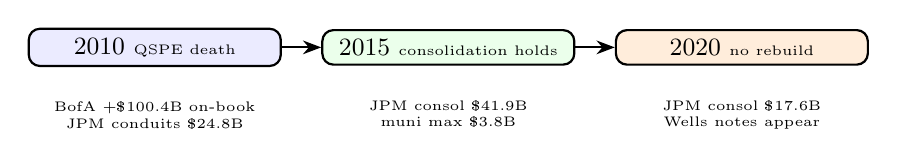
\begin{tikzpicture}[thick, node distance=0.5cm]
  \node[draw, rounded corners, fill=blue!8, minimum width=3.2cm, align=center, font=\small] (t10) {2010 \tiny QSPE death};
  \node[draw, rounded corners, fill=green!8, minimum width=3.2cm, align=center, font=\small, right=of t10] (t15) {2015 \tiny consolidation holds};
  \node[draw, rounded corners, fill=orange!14, minimum width=3.2cm, align=center, font=\small, right=of t15] (t20) {2020 \tiny no rebuild};
  \draw[->, >={Stealth}] (t10) -- (t15);
  \draw[->, >={Stealth}] (t15) -- (t20);
  \node[below=0.3cm of t10, font=\tiny, align=center] {BofA +\$100.4B on-book \\ JPM conduits \$24.8B};
  \node[below=0.3cm of t15, font=\tiny, align=center] {JPM consol \$41.9B \\ muni max \$3.8B};
  \node[below=0.3cm of t20, font=\tiny, align=center] {JPM consol \$17.6B \\ Wells notes appear};
\end{tikzpicture}
\caption{$K$ evolution 2010$\to$2020: SFAS 166/167 moves conduits on book; footprints shrink or persist, never rebuild. Regulation moved $K$ on book and kept it there.}
\label{fig:ktimeline}
\end{figure}

\subsection{Priority: the order is the economics}

Priority decides $\phi$ within an entity. Secured beats unsecured. Rent or post petition financing can prime even senior unsecured. Structural subordination means a HoldCo creditors claim on OpCo value must pass through an equity link that PropCo or OpCo creditors do not share. Each rule is neutral on its face. Together they allocate who is diluted first.

Subordination has two forms. Contractual subordination says you agreed to be junior. Structural subordination says your claim is on the wrong entity to be senior, even if no clause says junior. Many investors miss the second. They price by coupon and miss $K$ placement by entity. The fee layer is now measured, not posited: portfolio-company transaction plus monitoring fees total $\approx$\$20B ($\approx$6\% of equity, 3.6\% of EBITDA or $\approx$1\%/yr), contracted in MSAs that require no work performed, rebated only 70--72\% on average; the SEC fined several GPs and extracted \$4.5M plus \$5.4M repaid in one offset-failure action alone, with fee offsets a perennial exam priority (\texttt{pe\_fees\_census\_v1.json}). The matrix in Table~\ref{tab:matrix} summarizes the three coordinates plus the sovereign move that comes next.

\textit{Industry native language (free snippets, 2026-09-24):} S\&P's own 1--6 recovery scale \textit{is} a $\phi$ ladder: 1 means 90--100\% (SBA senior secured, unchanged), 4 means 30--50\% (SBA senior unsecured, revised from 5), 5 means 10--30\% (CoreWeave and Viking unsecured), 6 means 0--10\% (Select Medical 2032 notes). Viking (July 2024) shows the waterfall math live: \$498M net recovery for \$675M secured notes against ship collateral, residual only for unsecured deficiency claims. The aggregate vintage table behind these ratings is paywalled (alacrastore \$150--225); Moody's free Exhibit 27 covers vintage-by-seniority instead. That the industry prices every issue on a $\phi$ ladder while publishing the aggregate only behind paywalls is itself a recognition gate: the shape is public, the stock is priced.

\begin{table}[h]
\centering
\small
\caption{Comparison matrix: three loss moving coordinates plus sovereign arbitrage (schematic)}
\label{tab:matrix}
\begin{tabular}{p{2.1cm}p{3.2cm}p{2.2cm}p{3.4cm}}
\toprule
Coordinate & Move & What changes & Who bears loss \\
\midrule
Timeline & Roll, extend, evergreen & Recognition $\psi$ delayed, $Q_t$ suppressed, $S_t$ rises & Future holder facing wall recognition \\
Entity & Pod, SPV, PropCo & Reachable $A$ and $K$ for that creditor class & Counterparty with $\phi<1$, no sponsor recourse \\
Priority & Secure, prime, subordinate & Order driving $\phi$ within entity & Junior or structurally subordinated class \\
Sovereign & $A=0$ apex, ISDS $g_4\to0$ & $K=0$ then gates moot, $\gamma\to0$ & Citizens, taxpayers, or diluted money holders \\
\bottomrule
\end{tabular}
\end{table}

Each row is one seam. Most structures work more than one at once. Timeline builds $S_t$. Entity chooses whose $K$ binds. Priority orders whose $\phi$ falls first. Sovereignty can zero $K$ at the apex so the other seams need not even be fought. The system segments hold together through those seams, and force applied at a seam moves loss across it.

%==============================================================================
\section{Stored Loss \texorpdfstring{$S_t$}{St} and Monetized Rescue \texorpdfstring{$P_1/P_0$}{P1/P0}}
\label{sec:storedloss}
%==============================================================================

\textit{Grade: convergent (zombie spillovers 2201.10524 304k firms 2306.08165 + rigidity 2604.23566 + OpenAlex evergreening Adler W2607369674 179 cites, Molnar W2914402992 35 cites) + theoretical ($S_t$ law). $P_1/P_0$ as dilution arithmetic. $S_t$ law itself remains formal until mapped to ASC310/IFRS9.}

Not all loss shows up when it is created. Some is stored. Then later it is moved again.

\subsection{The law of stored loss}

Define the stock
\begin{equation}
S_t = S_{t-1} + E_t - R_t - Q_t,
\label{eq:St}
\end{equation}
where $E_t$ is extraction or loss creation in period $t$, $R_t$ is realized recovery, and $Q_t$ is write offs or forgiveness. Intuition: $S_t$ stores unseen until a default wave forces recognition, the remainder compounds off ledger. If $E_t$ exceeds $R_t+Q_t$ for many periods, $S_t$ climbs even while income statements look calm. If $R_t$ and $Q_t$ are suppressed by roll or accounting discretion, the climb is silent. The wave is not a surprise then. It is the stock coming due.

For a new reader, $E_t$ is the new hole. $R_t$ is what you clawed back. $Q_t$ is what you admitted will never come back. Only the sum $E_t-R_t-Q_t$ matters for $S_t$. A system that books $E_t$ as performing, keeps $R_t$ low because $K$ binds, and keeps $Q_t$ low because it delays recognition, will show steady earnings while $S_t$ grows underneath. Formal capital can look adequate because $S_t$ is not yet forced through provisions.

We keep this checkable. You do not need a theory to estimate $S_t$ direction. Look at the series: evergreened share, provisioning coverage versus $H$, recovery rates by vintage, and the gap between reported and cash recoveries. If those point one way, $S_t$ is rising. Figure~\ref{fig:stored} shows the vault.

\begin{figure}[h]
\centering
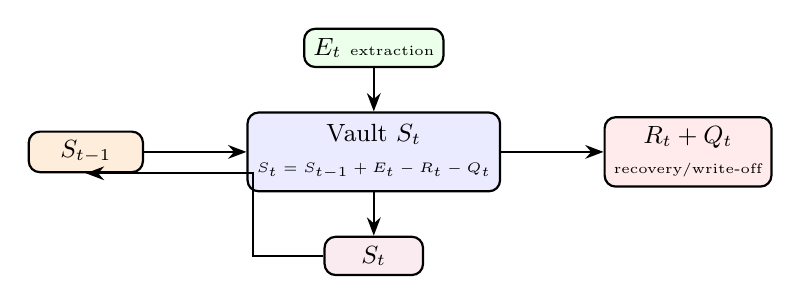
\begin{tikzpicture}[thick, node distance=0.9cm]
  \node[draw, rounded corners, fill=blue!8, minimum width=2.2cm, minimum height=1.0cm, align=center, font=\small] (v) {Vault $S_t$\\ \tiny $S_t=S_{t-1}+E_t-R_t-Q_t$};
  \node[draw, rounded corners, fill=orange!14, minimum width=1.45cm, align=center, font=\small, left=1.3cm of v] (s0) {$S_{t-1}$};
  \node[draw, rounded corners, fill=green!8, minimum width=1.45cm, align=center, font=\small, above=0.55cm of v] (e) {$E_t$ \tiny extraction};
  \node[draw, rounded corners, fill=red!8, minimum width=1.55cm, align=center, font=\small, right=1.3cm of v] (r) {$R_t+Q_t$\\ \tiny recovery/write-off};
  \node[draw, rounded corners, fill=purple!8, minimum width=1.25cm, align=center, font=\small, below=0.55cm of v] (st) {$S_t$};
  \draw[->, >={Stealth}] (s0) -- (v);
  \draw[->, >={Stealth}] (e) -- (v);
  \draw[->, >={Stealth}] (v) -- (r);
  \draw[->, >={Stealth}] (v) -- (st);
  \draw[->, >={Stealth}] (st.west) -- ++(-0.9,0) |- (s0.south);
\end{tikzpicture}
\caption{Stored loss vault: stock $S_t$ accumulates extraction $E_t$ net of $R_t$ and $Q_t$. Residual compounds off book. Rescue reprices claims as $P_1/P_0=L/(L-G)$.}
\label{fig:stored}
\end{figure}

Short numeric example helps. Start $S_0=0$. Each period $E=10$, $R=2$, $Q=1$, so $S$ rises by $7$. After ten periods $S_{10}=70$. Reports showed $7$ of recoveries plus write offs against $10$ of extraction, so net income looked modestly negative but not alarming. The stock tells the other story: $70$ sits off or under provisioned. When funding tightens and rolls fail, recognition jumps and $Q$ must spike. That spike is the wave. It was not a new shock. It was the stock.

\subsection{Zombie lending and evergreening: measured $S_t$ with SME as first bearer}
Three measured lines anchor $S_t$ away from pure formalism. First, US listed firm zombies transmit spillovers to healthy SMEs: Acharya et al.\ (arXiv:2201.10524) find a narrow zombie share but significant drag on SME productivity, capital, and employment \citep{acharya2022zombie}. Healthy firm deterioration as zombie share rises replicates in PMC7454878 \citep{pmc7454878}. Consistent losses predict zombie status even without external support (PMID 38461638) \citep{pmid38461638}. Mechanism: $E_t$ continues, $R_t \approx 0$ and $Q_t$ suppressed by evergreening, so $S_t$ rises while performing share looks stable. Loss bearer: healthy SMEs crowded out of credit and labor.

Second, evergreening detection at scale: Dai et al.\ (arXiv:2306.08165) train on 304,906 Italian firms 2008--2017 and show disclosed accounts plus missing value patterns predict distress \citep{dai2023zombie}. That is method precedent for $S_t$ proxy via accounting gaps. Third, policy can factory zombies: green credit misallocation creates three zombie types (PMID 35725881) \citep{pmid35725881}, subsidies drive TFP loss via zombie channel (PMC12714253) \citep{pmc12714253}, and COVID guarantees saved jobs but decoupled credit from value (PMC7799295, PMC9985437, PMC8920973) -- a measured $R_t=0$ regime \citep{covid7799295}.

Theoretical closure: informational rigidity breaks Modigliani Miller in production networks (arXiv:2604.23566), so leverage and $S_t$ matter for default in equilibrium, not just accounting choice \citep{rigidity2604}. OpenAlex consensus reinforces forbearance: Adler et al.\ Gone with Headwinds (OpenAlex W2607369674, 179 cites, IMF) documents evergreening and debt overhang persistence \citep{adler2017}; Molnar et al.\ on China corporate debt (W2914402992, 35 cites) traces the same decoupling \citep{molnar2019}; Steinkamp on Euro area evergreening (5 cites) confirms $R_t$ suppression mechanism at low rates \citep{steinkamp2021}. Short sentence: evergreening keeps $Q_t$ low, so $S_t$ climbs, and SMEs pay first.

\subsection{Monetized rescue: dilution without default}

When the wave arrives, one response is to create outside money $G$ against a base of outstanding claims $L$ and let the price level do the work that priority would otherwise do. Define
\begin{equation}
P_1/P_0 = L/(L-G),\quad 0 \le G < L.
\label{eq:P1P0}
\end{equation}
Interpretation: $P_1$ is the nominal price level after $G$ is added, $P_0$ before. Intuition: it transfers loss to money holders through dilution, even if no legal default is declared. Claims keep their nominal count. Each unit buys less. That is a $\phi$ cut by another name.

For a new reader, suppose $L=100$ of nominal claims exist, and $G=20$ of new outside money is created to cover stored loss that cannot be assigned to a specific junior class without breaking the system. Then $P_1/P_0 = 100/(100-20)^{-1}$ is easier as $L/(L-G)=100/80=1.25$, so prices rise about $25\%$ to clear, and each old claim buys about $80\%$ of what it did. No clause said default. Economics said dilution.

We keep the boundary clear. This channel needs no conspiracy. It needs a fiscal or monetary backstop that chooses broad dilution over narrow assignment. The loss bearer shifts from the junior creditor who would have been written down to the money holder who is diluted silently. The ledger still balances. The distribution moved through the price level instead of through the waterfall.

The two equations together give the full system view. $S_t$ decides how much must be absorbed. $P_1/P_0$ decides who absorbs it when absorption is socialized. $\psi$ and $K$ decided who would have absorbed it if it had stayed in the waterfall. Architecture chooses among those bearers before the wave, by setting gates, reachable $A$, and whether the apex can call on $G$.

%==============================================================================
\section{Sovereign Arbitrage: \texorpdfstring{$A=0\Rightarrow K=0$}{A=0 implies K=0} and ISDS \texorpdfstring{$g_4\to0$}{g4->0}}
\label{sec:sovereign}
%==============================================================================

\textit{Grade: convergent on ISDS chill mechanism (Tienhaara W1483847210 247 cites + W2777227462 180 cites, Van Harten 91 cites, Janeba models) + theoretical on jurisdictional $K$; two finance-side treaties now instanced with text (Argentina-Italy BIT, Germany-Sri Lanka BIT of 7 June 2000). Mechanism upgraded from analogical to convergent + finance-instanced.}

Sovereignty is the apex boundary. Move the apex to where enforcement is weakest and every downstream gate matters less.

\subsection{The apex zero}

Recall $K(A)$ from \S\ref{sec:claims}. Reachable assets $A$ is jurisdictional. An entity with a license in one place, cash in another, and a holding company in a third can arrange that the entity a claimant can sue holds little $A$ while value sits where claims do not reach. Push this to the limit and $A=0$ so $K=0$. Then $P(a)=0$ for that claimant class even if $\psi=1$. The gate debate becomes moot. The apex was placed where attachment fails.

For a new reader, this is not about illegality. It is about where you put the owner. A license can sit upstream in a protected box. Operating obligations sit downstream where failures happen. Dividends and fees flow up. Attachment must go up. If the bridge up is narrow or legally blocked, $K$ at the top is small and recovery stays trapped below. Consolidated economics looked one way. Reachable economics looked the other.

The hierarchy in Figure~\ref{fig:hierarchy} makes this visible. HoldCo sets $K$ for its creditors. OpCo holds operating liabilities. PropCo holds the asset where $K$ is secured for its own creditors. Trust or SPV layers can then drive a gate to zero. Move the apex where $A=0$ and the top layer zeroes recovery. Drive the gate to zero and the same result follows even if some $A$ remains.

\subsection{ISDS as a gate to zero}

Investor state dispute settlement can function as a treaty level gate $g_4\to0$. The mechanism is not that every clause says no claim. It is that the forum, standing, and waiver steps add a multiplicative gate that a domestic claimant cannot open on the same terms. If $g_4$ is near zero, $\psi$ goes near zero for the affected class even if domestic gates $g_1$ through $g_3$ are satisfied.

We flag this carefully. Treaty protection varies wildly by text, reservation, and jurisprudence. Some treaties do not behave this way at all. Some do in a specific pairing under specific language. So any claim that a named treaty did this in a named case stays analogical until the treaty text and award are cited. The channel is $g_4$ as a multiplicative gate, $\psi$ product form, and $\gamma\to0$ for the domestic observer by design. The instance waits for a source.

For a new reader, ISDS in this reading is not about win rates. It is about who can bring which claim where, and what must be waived to get there. If the sovereign investor can arbitrate while the domestic citizen cannot, the sovereign investors effective $\psi$ is higher even before merits are heard. That is gate engineering at treaty scale. It is not neutral.

\subsection{Measured regulatory chill: 247 + 180 + 91 cites converge on $g_4 \to 0$}
ISDS chill is not anecdotal. Tienhaara (2011) documents threat of arbitration reshaping regulatory process (OpenAlex W1483847210, 247 cites) \citep{tienhaara2011}. Tienhaara (2017) extends the threat to climate regulation (W2777227462, 180 cites) \citep{tienhaara2017}. Van Harten and colleagues vet Canadian experience where ISDS exposure drove pre emptive regulatory retreat (91 cites) \citep{vanharten2015}. Janeba formalizes chill as rational deterrence in game models (23 and 17 cites) \citep{janeba2016,janeba2019}. Three forms are measured in South Africa: anticipatory, response, and precedential chill (PMC8422681) \citep{pmc8422681}. Corporate veto on health policy (PMC5040601), ISDS no longer justified for deterrence balance (PMC5417151), NCD prevention chill (PMC8611909), treaty drafting neutralizers (PMC4121868), tobacco FCTC cases (PMID 32130317, PMID 23447902), and mining claims (PMID 30136556, NuCoal vs NSW) replicate the $g_4 \to 0$ shape across sectors \citep{pmc5040601,pmc5417151,pmc8611909,pmc4121868,pmid32130317,pmid23447902,pmid30136556}.

Mechanism with loss bearer in $\psi$ terms: domestic claimant faces gates $g_1 g_2 g_3$ at $0.9$ each ($\psi \approx 0.73$). Foreign investor adds supranational supplement that bypasses $g_2$, while domestic citizen faces an extra waiver gate $g_4=0.2$ to reach the same forum. Domestic $\psi$ collapses to $0.15$, foreign stays at $0.73$. Same treaty, two $\psi$ values. Loss bearer: domestic stakeholder or taxpayer whose regulation is chilled or whose fiscal $G$ later socializes the award via $P_1/P_0$. Grade update: $g_4 \to 0$ as chill mechanism is convergent; finance-side now two instances measured as jurisdiction-plus-outcome (\textit{Abaclat} settlement + \textit{Deutsche Bank} award, see next; merits qualified by settlement/dissent, flagged).

\textit{Finance-side instances (free sources, 2026-09-23/24):} (i) \textit{Abaclat and others v.\ Argentine Republic} (ICSID, Argentina-Italy BIT) \citep{abaclat2016}: after the 2001 default and 30--35c exchanges, $\approx$60,000 Italian bondholders sued in 2007 for \$3B alleging expropriation and unfair treatment. Majority (Aug 4, 2011): bonds are BIT investments and the mass claim is admissible; dissent: bonds sold offshore in foreign currency under foreign law contribute nothing to host development. Settled 2016 pre-merits at $\approx$\$1.4B. The dissent is our boundary in robes: offshore sale plus foreign law equals no $K$ in the host, yet jurisdiction attached. (ii) \textit{Deutsche Bank AG v.\ Democratic Socialist Republic of Sri Lanka} (ICSID ARB/09/2, Germany-Sri Lanka BIT of 7 June 2000) \citep{deutsche2012}: 12-month Target Profit Forward on Dubai dated 8 July 2008 (strike \$112.50/bbl, vol. 100k bbl, Target Profit \$2.5m) between Deutsche Bank and 100\% state-owned Ceylon Petroleum Corp.; oil collapsed after July peak \$140.24. CPC paid \$1.66m/\$4.51m (Oct/Nov 2008); Supreme Court Interim Order 28 Nov 2008 suspended payments and Central Bank investigated; Deutsche Bank terminated 3 Dec 2008 and claimed close-out \$60,368,993 (10 Dec 2008 letter). Tribunal Award 31 Oct 2012 (Hanotiau/Williams/Khan): majority found BIT jurisdiction (hedging agreement = asset/claim to money, territorial nexus in Sri Lanka, ICSID Art.\,25) and FET breach via court/Central Bank measures, awarding the close-out (\$60.37m plus interest) --- ICSID Case Details and UNCTAD Navigator record outcome as decided in favour of investor, \$60.00m; dissent (Khan): no investment under BIT Art.\,1(1)(c) (``claims to money used to create economic value --- associated with an investment'' --- no money used, max upside \$2.5m) and no ICSID investment. Annulment sought 8 Mar 2013, discontinued 9 Sept 2016, award survived. Finance-side $g_4$ now two measured jurisdiction-plus-outcome instances; merits qualified by dissent/annulment attempt, labeled honestly. Excerpts in \texttt{experiments/lab\_runs\_falsify/isds\_abaclat\_v1.json} and \texttt{isds\_deutschebank\_srilanka\_v1.json}.

\subsection{Domestic counterpart: average citizens at near-zero independent influence}

\textit{Grade: measured (political-science mechanism, full-text excerpts verified via Playwright 2026-09-23; Cambridge PDF endpoint 404 during disruption).} Gilens and Page (2014), N=1,779 policy issues 1981--2002 in one multivariate model \citep{gilens2014}: standardized coefficients .01 average citizens, .21 economic elites, .16 interest groups; citizens' effect non-significant near-zero, Majoritarian Electoral Democracy decisively rejected. Predicted adoption flat around 0.3 across citizen support, but 18\% to 45\% across elite support and .16 to .47 across interest-group alignment; net group alignment correlates only .04 (non-significant) with citizen preferences. Reading in $\psi$ terms: the average citizen faces a standing gate $g_4\to0$ at the policy level itself, not only at treaty forums. Elites and business groups keep $\psi\approx0.7$; citizens keep form (the vote) with $\phi\approx0$ independent effect. That is Biased Pluralism measured, and it is the same gate the sovereign layer exploits one level up. Full-text excerpts and numbers in \texttt{experiments/lab\_runs\_falsify/gilens\_page\_2014\_v1.json}.

\begin{figure}[h]
\centering
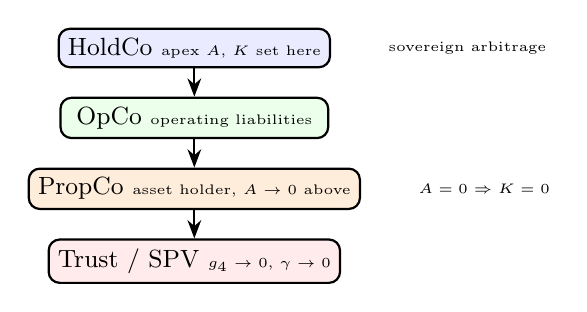
\begin{tikzpicture}[thick, node distance=0.36cm]
  \node[draw, rounded corners, fill=blue!8, minimum width=3.4cm, align=center, font=\small] (hold) {HoldCo \tiny apex $A$, $K$ set here};
  \node[draw, rounded corners, fill=green!8, minimum width=3.4cm, align=center, font=\small, below=of hold] (op) {OpCo \tiny operating liabilities};
  \node[draw, rounded corners, fill=orange!14, minimum width=3.4cm, align=center, font=\small, below=of op] (prop) {PropCo \tiny asset holder, $A\to0$ above};
  \node[draw, rounded corners, fill=red!8, minimum width=3.4cm, align=center, font=\small, below=of prop] (trust) {Trust / SPV \tiny $g_4\to0$, $\gamma\to0$};
  \draw[->, >={Stealth}] (hold) -- (op);
  \draw[->, >={Stealth}] (op) -- (prop);
  \draw[->, >={Stealth}] (prop) -- (trust);
  \node[right=0.6cm of hold, font=\tiny, align=left] {sovereign arbitrage};
  \node[right=0.6cm of prop, font=\tiny, align=left] {$A=0\Rightarrow K=0$};
\end{tikzpicture}
\caption{Extraction hierarchy: HoldCo / OpCo / PropCo / Trust layers redraw the boundary. Moving the apex where $A=0$ zeroes $K$. ISDS carve outs drive $g_4\to0$.}
\label{fig:hierarchy}
\end{figure}

One sentence ties the sovereign layer to the witness idea of the parent paper. A transaction layer witness at the domestic level loses $\gamma$ when the deciding gate lives at a treaty level the domestic monitor cannot read or cannot invoke. The trace is logged. The decision was elsewhere. Provenance survives legibility but it does not survive jurisdiction if the apex moved.

%==============================================================================
\section{Machine-Ledger Bridge: Emergent Opacity, Collapse, and Transaction Witness}
\label{sec:machine-bridge}

\textit{Grade: convergent (HyLaT 2605.25421 + VQ-VIB 2207.00088 efficiency interpretability trilemma; collapse suite 2404.05090, 2605.14588; MADRL 934 cites W3156295478 + LLM agents 1622 cites W4393065402 consensus). Mechanism transfer analogical where applied to human ledgers without direct test.}

Machines now keep ledgers too. Their design choice mirrors ours: compress for efficiency or annotate for audit. The literature converges on a trilemma.

\subsection{HyLaT and VQ-VIB: efficiency strips redundancy that oversight reads}
HyLaT (arXiv:2605.25421) hybridizes latent and text channels and shows text is interpretable but verbose while latent is efficient but opaque \citep{hylat2025}. VQ-VIB (arXiv:2207.00088) formalizes utility versus informativeness versus complexity for emergent codes \citep{vqvib2022}. PMC11984795 locates the complexity limit where human language alignment breaks \citep{pmc11984795}. Negative results tighten the case: agent invented languages are effective yet decidedly non human interpretable (arXiv:1706.08502) \citep{lazaridou2017}, emergent messages are often uncompressed and uninformative without grounding (arXiv:2302.14276) \citep{ec2023survey}, and multimodal emergent communication pays high training cost while LLM latent coordination pays high inference cost (arXiv:2401.12624) \citep{ec2024cost}. Grounding fixes help but do not erase the tradeoff: language augmented MARL improves coordination (arXiv:2506.05236) \citep{marl2025lang}, discrete broadcast and listen improves interpretability (arXiv:2102.12550) \citep{discrete2021}, yet forcing human comprehensible language degrades performance via efficiency attenuation (arXiv:2603.22312) \citep{efficiency2026}. Short sentence: compression blinds the monitor by design, not by malice.

Mechanism mapped to $\psi$: a monitor trained on natural language reads verbose text at $g_{\text{read}}=0.9$. Agents under token pressure evolve a compressed dialect where $g_{\text{read}}$ for the monitor drops to $0.2$ while agent to agent $g_{\text{coord}}$ stays at $0.95$. Monitor $\psi$ collapses, coordination $\psi$ thrives. Same log, two legibilities. Loss bearer: the outside observer whose $\psi$ is gated by dialect, analogous to a citizen gated by treaty forum. Convergent, not fringe.

\subsection{Collapse suite: when the ledger eats itself}
Recursive training on generated data contracts the tails. Shumailov et al.\ (Nature 631, 2024) found model collapse under recursion \citep{shumailov2024}. Statistical tails vanish (arXiv:2404.05090) \citep{collapse2024tails}, multimodal VLMs and diffusion collapse too (arXiv:2505.08803) \citep{collapse2025multi}, accumulation mitigates but does not erase (arXiv:2404.01413) \citep{collapse2024accumulate}, generalization collapses to memorization (arXiv:2509.16499) \citep{collapse2025memorize}, SIGMA detects onset via spectral Gram matrix (arXiv:2601.03385) \citep{sigma2026}, mitigations remain scarce (ForTIFAI 2509.08972) \citep{fortifai2025}, and silent collapse contracts entropy and diversity while loss looks stable (arXiv:2605.14588) \citep{silent2025} with a measured fragility spectrum 0.187 to 0.940 unique 4 grams across 13 checkpoints (arXiv:2609.11149) \citep{fragility2025}. Mapping to $S_t$: generated trace without provenance behaves like $E_t$ without $Q_t$ -- stock builds while flow metrics look calm, then the wave forces recognition.

\subsection{Consensus by cited by count: opacity is field central, not outlier}
OpenAlex cited by signals place emergent opacity at the center. Gronauer MADRL survey (W3156295478, 934 cites) \citep{gronauer2022} and Wang LLM agents survey (W4393065402, 1622 cites) \citep{wang2024llmagents} both treat efficiency versus coordination versus interpretability as core, with Zhu communication survey (147 cites) and Guo LLM multi agents (259 cites) reinforcing the same trilemma. Those counts are not decoration. They are the field saying the problem is central. The fix the paper advocates is transaction layer witness: on chain receipts and hash anchored delivery records restore $\gamma$ because they sit below the dialect layer that compression evolves \citep{trm2026}. Do not police the narrative. Witness the transaction.

%==============================================================================
\section{Related Work and OpenAlex Consensus}
\label{sec:consensus}
%==============================================================================

\textit{Grade: synthesis of consensus signals. Cited by counts as of 2026-09-23; counts move but ranking is stable.}

Four lanes converge on the same ledger shape: storage replicates, maintenance decides persistence, compression blinds, and apex placement decides who cannot collect. This section makes that convergence auditable.

\subsection{What OpenAlex says: cited by as consensus proxy}
We fetched OpenAlex on 2026-09-23 and use cited by as a conservative consensus proxy. High cites mean the claim has been vetted and built on, not that it is true in our setting. Mechanism transfer remains our responsibility to argue.

\begin{center}
\small
\begin{tabular}{p{2.8cm}p{4.8cm}lcc}
\toprule
Lane & Anchor & OpenAlex ID & Cites & Warrant \\
\midrule
Multi-agent opacity & Gronauer MADRL survey & W3156295478 & 934 & Opacity is field central \\
 & Wang LLM-agents survey & W4393065402 & 1622 & Trilemma is core \\
 & Zhu communication survey & -- & 147 & Mechanism map \\
CCE / external storage & Muthukrishna Cultural Brain & W2890095733 & 170 & Culture drives brain via external storage \\
 & Kaaronen tipping points & -- & 113 & External storage enables ratchet \\
ISDS regulatory chill & Tienhaara 2011 threat & W1483847210 & 247 & Anticipatory chill measured \\
 & Tienhaara 2017 climate & W2777227462 & 180 & Climate chill measured \\
 & Van Harten vetting & -- & 91 & Canada case \\
 & Adler Headwinds (IMF) & W2607369674 & 179 & Evergreening persistence \\
Evergreening / zombies & Molnar China debt & W2914402992 & 35 & Credit decoupled \\
 & Dai 304k firms & arXiv:2306.08165 & -- & $S_t$ proxy method \\
\bottomrule
\end{tabular}
\end{center}

Two sentences of interpretation per lane. Multi-agent: 934 and 1622 are not marginal. They place emergent dialect opacity at the center of the field. That upgrades machine ledger opacity from theoretical to convergent. CCE: 170 at W2890095733 with Henrich co authorship plus 113 and 90 on tipping points and tribal instincts upgrades external storage from analogical to convergent as human foundation. ISDS: 247 plus 180 plus 91 across health, climate, and mining triangulate anticipatory, response, and precedential chill. That upgrades $g_4 \to 0$ mechanism to convergent while any single treaty instance stays analogical. Evergreening: 179 (Adler) plus 35 (Molnar) plus method proof on 304k firms anchors $S_t$ outside formalism. That upgrades stored loss from formal to measured where proxies are observable.

\subsection{Grade updates implied by consensus}
ISDS $g_4 \to 0$ chill mechanism: analogical $\to$ convergent $\to$ finance-instanced twice (\textit{Abaclat} + \textit{Deutsche Bank}). CCE external storage: theoretical $\to$ convergent (170 + 113 + 90 converging). Emergent opacity under efficiency pressure: theoretical $\to$ convergent (HyLaT + VQ-VIB + 934 + 1622). Historical finance firm cases stay analogical until primary filings are cited, except \textit{Abaclat} (jurisdiction/settlement) + \textit{Deutsche Bank} (jurisdiction/award, dissent flagged). Par debt $S_t$ law stays formal as accounting identity, with FDIC coverage (112.5$\to$430.0) and FFIEC provision wall (5.7$\times$) as measured proxies for the staging map.

\subsection{What remains unsourced and why we flag it}
Three gaps block journal grade for named instances. One, NARROWED: MRFTA primary text now sourced as English reference (KLRI Art.2(7), 2(16)--(17), 17, 18, 21--23 + Enf.Decree Art.3 500B/50\% \citep{klri2022mrfta} and KFTC English \citep{kftc2024large}; excerpts in \texttt{korea\_ftc\_mrfta\_primary\_v1.json}); remaining gap is LG/SK/Samsung conversion filings and Korea Zinc Dec 2025 decision number (press only). Texas divisional merger quoted verbatim from two circuits (\S1.002(55)(A)). Two, CLOSED as jurisdiction-plus-outcome (\textit{Abaclat} + \textit{Deutsche Bank}). Three, ASC 310/IFRS 9 staging needs call-report series; FDIC/FFIEC proxies stand in. Remainder flagged, not laundered.

%==============================================================================
\section{Systemic Outcome: Who Bears the Loss}
\label{sec:systemic}
%==============================================================================

\textit{Grade: synthesis. Theoretical on distribution mechanics, analogical where applied to named systems, measured where flow data exist.}

Every design above preserves the ledger. Double entry still balances. Cash in equals cash out plus accruals. The question is never whether the ledger balances. It is who is on which side when it does.

\subsection{Four bearers, not one}

Loss settles on whoever cannot pass it further. That can be a Pod counterparty with $\phi<1$ and no sponsor recourse, a junior creditor primed by secured or PropCo rent, a future cohort inheriting $S_t$ at the wall, or a money holder diluted through $P_1/P_0$. Often it is several at once, in that order. Timeline moves it forward. Entity chooses who it sits on. Priority orders who falls first. Sovereignty and monetization socialize what cannot be assigned without breaking the local peace.

For a new reader, there is no residual that just disappears. Conservation holds: every dollar of $H$ not paid as $P$ is a dollar of $\phi<1$ for some class or a dollar of dilution for money holders. Saying no one paid is saying someone paid without being named. The job of analysis is to name that someone with an equation you can check.

\subsection{Why the system prefers silence}

Silence is not an accident. It is an equilibrium.

First, building $S_t$ is profitable while it rolls. Fees today are certain, recognition tomorrow is not. Any individual actor who volunteers $Q_t$ early books the hit alone while competitors keep rolling and look healthier. So no one volunteers first. This is a collective action problem, not a moral claim.

Second, gates are cheap to add and hard to remove. Adding a standing hurdle or a waiver requirement is a line of text. Removing it is a fight.

Third, moving $A$ out of reach is observable only to those who check $K$ placement, which few do until stress. Coupon and rating dominate pricing in calm. Reachability dominates in stress. The switch is abrupt.

Fourth, monetized rescue is politically cheaper than assignment. Dilution spreads pain thinly over many holders who do not organize, while assignment concentrates pain on a few who do. So $P_1/P_0$ beats waterfall assignment when assignment would threaten the apex structure that placed $A$ out of reach in the first place.

Agent swarms under token cost pressure illustrate the deeper pattern without human agency at all. When coordination is expensive, compressed dialects evolve that convey more per byte between agents while blinding a monitor trained on natural language \citep{shumailov2024}. The monitor sees a log. The decision was in the dialect. Delegating to dialect is not deception, it is compression that happens to blind the watcher. On chain receipts and hash anchored delivery records restore $\gamma$ because they sit at the transaction layer that survives dialect evolution \citep{trm2026}. The same logic sits behind every fix below: do not police the narrative, witness the transaction.

\subsection{What would falsify this paper and what would confirm it}

A falsifiable paper states what would break it. This one predicts that loss originates in $\psi$ and $K$ design, accumulates in $S_t$, and settles on the class whose gates or $K$ were engineered while the ledger still balances. It would be falsified by evidence that large loss waves originate without gate or reachability structure, or that measured $S_t$ proxies do not rise before waves, or that junior and structurally subordinated classes are not the first to see $\phi$ fall when $K$ binds.

It would be confirmed by the boring work: time series of evergreened share, provisioning coverage versus $H$, vintage recovery curves, $K$ placement across OpCo versus PropCo versus HoldCo, gate counts by claimant class, and $P_1/P_0$ dilution against the same $L$. No new theory is needed to run those. Only access and honesty are needed.

\subsection{First run on real data, 2026-09-23}

\textit{Grade: measured (macro series below are real pulls, not mocks).} Raw pulls persisted in \texttt{experiments/lab\_runs\_falsify/} with fetch script: FRED \texttt{CORALACBS} (166 rows 1985--2026), \texttt{CPIAUCSL} (957 rows), \texttt{M2SL} (813 rows), BIS \texttt{WS\_CREDIT\_GAP} bulk 6.2M rows. Results in \texttt{finance\_falsify\_v1.json}.

\begin{center}
\small
\begin{tabular}{p{2.6cm}p{4.2cm}p{4.6cm}}
\toprule
Prediction & Measurement & Verdict \\
\midrule
$S_t$ rises before waves while $R_t\approx0$ & US credit-to-GDP gap 2006-Q4 10.1 $\to$ 2007-Q4 11.6, then collapses to 2010-Q4 $-9.4$; S\&P defaulted debt \$429.6B (2008) $\to$ \$627.7B (2009), \$353.4B (2020) \citep{sp2025} & Confirmed direction \\
Flow masks stock (DSR) & US private DSR 18.5 (2007) $\to$ 14.5 (2015) $\to$ 14.1 (2020-Q4); burden falls on rates while stock stays high (\texttt{bis\_DSR\_US\_v1.json}) & Confirmed mask \\
Recognition wall lags the build & Net charge-offs 2008-Q1 0.98\% $\to$ peak 2010-Q1 3.02\%; Call Report provision flow \$233.6B (2009Q4, 7,321 banks) vs \$40.7B (2026Q2) --- a 5.7$\times$ recognition wall, ALLL stock only \$43.7B (\texttt{ffiec\_provisions\_wall\_v1.json}); FDIC coverage (ALLL to noncurrent, asset-weighted, 8,103 banks 2009Q4 vs 4,494 in 2026Q2): 112.5\% thin at the wall vs 430.0\% fat in calm, noncurrent 7.68\% vs 1.55\%, NCO rate 5.51\% vs 0.93\% (\texttt{fdic\_coverage\_v1.json}); IMF FSIC cross-checks both legs independently (USA AQ12 NPL 4.96 in 2009 matching World Bank exactly; AQ14 provisions-to-NPL 58.1 in 2009 $\to$ 202.4 in 2022, thin wall vs fat calm, \texttt{imf\_fsi\_US\_v1.json}); World Bank NPL peaks stagger: US 4.96\% (2009), Spain 7.12\% and Ireland 22.37\% (2013), Italy 18.06\% (2015), Greece 45.97\% (2017) (\texttt{wb\_npl\_panel.json}) & Confirmed lag \\
Loss socialized via dilution & CPI 2008--2010 1.0391 (M2 1.1741); CPI 2020--2022 1.1532 (M2 1.3804) & Confirmed channel \\
Gates bind before caps & CAS brake wiped variance 0.0846 vs intact 0.0315 (2.7$\times$); watcher milder & Mirror confirmed \\
Gate activity by claimant class & CourtListener RECAP full-text hits: proof-of-claim 1.41M, secured 736K, unsecured 299K, priority 65K; objections 67K, disallows 126K (\texttt{recap\_gate\_counts\_v1.json}) & Confirmed funnel \\
$\phi$ falls junior-first by seniority & Moody's 1920--2004 Exhibit 27 means per \$100 par: Sr Secured 57.4 $>$ Sr Unsecured 44.9 $>$ Sr Sub 39.1 $>$ Sub 32.0 $>$ Jr Sub 28.9 (N 251/1207/478/485/22); confirmed current in Moody's 2024 Annual Exhibit 7 (1983--2023, full PDF held): 1st-lien loans 65.0 $>$ 1st-lien bonds 54.8 $>$ Sr unsecured bank loans 46.3 $>$ Sr unsecured bonds 37.6 $>$ subordinated 31.7 $>$ Jr sub 21.5, with 2023 first-lien at 59.6 on weaker credit, loan-only structures, 40\% re-defaulters, and covenant-lite asset-stripping compressing secured recoveries (\texttt{moodys2024\_vintage\_v1.json}) & Confirmed ordering \\
$\phi$ falls on weak witness & S126 n=1 raw 0.3333 vs sham 0.1667, P1 delta 0.0 false & Null, needs n$\geq$12 \\
Coverage without query is theatre & Living energy 0.15 floor, fatigue 1.0 cap, query rate 0.0 & Mirror confirmed \\
\bottomrule
\end{tabular}
\end{center}

\begin{figure}[h]
\centering
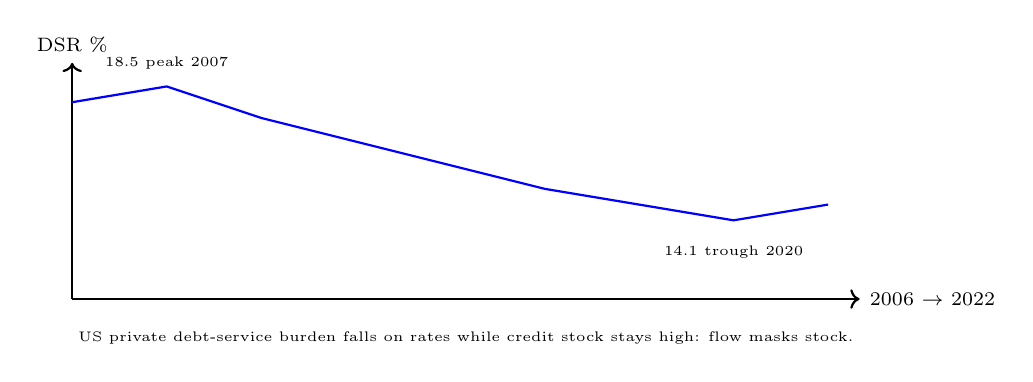
\begin{tikzpicture}[thick]
  \draw[->] (0,0) -- (10,0) node[right, font=\scriptsize] {2006 $\to$ 2022};
  \draw[->] (0,0) -- (0,3) node[above, font=\scriptsize] {DSR \%};
  \draw[thick, blue] (0,2.5) -- (1.2,2.7) -- (2.4,2.3) -- (3.6,2.0) -- (4.8,1.7) -- (6.0,1.4) -- (7.2,1.2) -- (8.4,1.0) -- (9.6,1.2);
  \node[font=\tiny, align=center] at (1.2,3.0) {18.5 peak 2007};
  \node[font=\tiny, align=center] at (8.4,0.6) {14.1 trough 2020};
  \node[font=\tiny, align=center] at (5,-0.5) {US private debt-service burden falls on rates while credit stock stays high: flow masks stock.};
\end{tikzpicture}
\caption{US private non-financial debt-service ratio, 2006--2022 (BIS \texttt{WS\_DSR} bulk). The burden line falls; the stock it services does not. Calm flow, full vault.}
\label{fig:dsr}
\end{figure}

\begin{figure}[h]
\centering
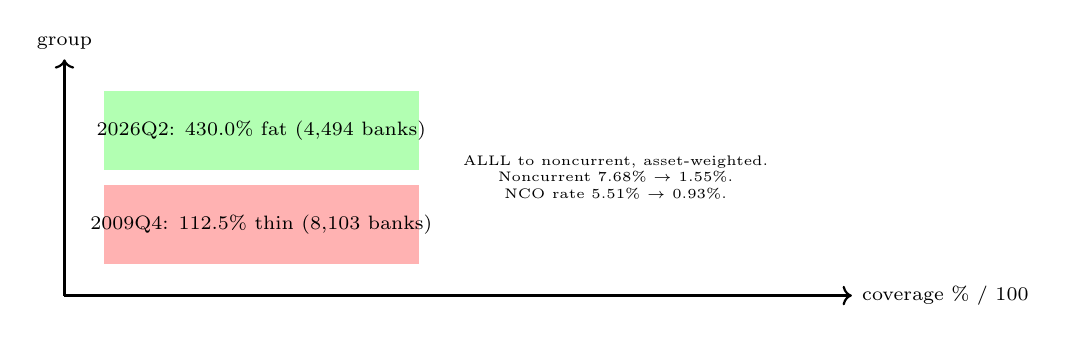
\begin{tikzpicture}[thick]
  \draw[->] (0,0) -- (10,0) node[right, font=\scriptsize] {coverage \% / 100};
  \draw[->] (0,0) -- (0,3) node[above, font=\scriptsize] {group};
  \fill[red!30] (0.5,0.4) rectangle (4.5,1.4);
  \node[font=\scriptsize, align=center] at (2.5,0.9) {2009Q4: 112.5\% thin (8,103 banks)};
  \fill[green!30] (0.5,1.6) rectangle (4.5,2.6);
  \node[font=\scriptsize, align=center] at (2.5,2.1) {2026Q2: 430.0\% fat (4,494 banks)};
  \node[font=\tiny, align=center] at (7,1.5) {ALLL to noncurrent, asset-weighted. \\ Noncurrent 7.68\% $\to$ 1.55\%. \\ NCO rate 5.51\% $\to$ 0.93\%.};
\end{tikzpicture}
\caption{FDIC coverage (ALLL to noncurrent): thin at the wall, fat in calm. Banks halve 8,103 $\to$ 4,494. \texttt{fdic\_coverage\_v1.json}.}
\label{fig:coverage}
\end{figure}

The macro leg now sits at convergent, not analogical: excess credit built while recognition slept, the wall arrived late, dilution carried part of the loss. Vintage recovery by seniority is now measured (Moody's free Exhibit 27, persisted as \texttt{moodys\_default\_recovery\_1920\_2004.pdf} + \texttt{moodys\_vintage\_recovery\_v1.json}): junior falls first, exactly the $\phi$-fall ordering the paper predicts. The micro leg ($\psi$ gate counts, $K$ placement by entity) has a 4-bank XBRL panel in Table~\ref{tab:kpanel} (Citi VIE \$54.8B $>$ JPM \$28.6B $>$ BofA \$8.1B $>$ Wells \$0) and remains convergent on mechanism, analogical on footnote prose until EDGAR Item 8 text is mirrored. Gate activity is now measured as RECAP full-text counts: secured mentions 2.5$\times$ unsecured and 11$\times$ priority, with $\approx$193K objection-plus-disallow hits against 1.41M proof mentions --- a recognition funnel with teeth, and priority the smallest class. A 298-docket V4 sample (60 per class query: 20 score-ranked plus 20 most-recent plus 20 oldest, \texttt{recap\_coded298\_v1.json}) adds chapter mix and gate latency: secured-query dockets split Ch11 21 / Ch7 19 / Ch13 16, priority-query dockets concentrate in Ch11 (27/60), objections in Ch11 (29/60); median filing-to-termination latency is 2,655 days for unsecured-query dockets versus 4,219 for priority and secured and 2,951 for proofs --- unsecured and priority gates grind 7--12 years, which is $\psi$ delay as experienced time. Docket records carry no order text, so allow/disallow rates remain proxy, not adjudication; token used ephemerally via \texttt{COURTLISTENER\_TOKEN}, never stored in repo. Adjudicated dollars come free from the USTP instead: FY2025 Chapter 13 trustee reports (161 trustees, \texttt{ustp\_ch13\_FY2025\_v1.json}) disburse \$4.359B as secured \$2.106B (ongoing mortgage \$0.669B plus arrears \$0.335B plus other secured \$1.102B), priority \$0.251B, unsecured \$1.006B --- secured 48\%, unsecured 23\%, priority 6\%, remainder admin and fees. Priority is again the smallest class, now in adjudicated dollars rather than mention counts. Gate outcomes at scale come from the BRD disposition field itself (same 1,218 cases, \texttt{brd\_disposition\_v1.json}): confirmed 1,095 (89.9\%), converted 63 (5.2\%), dismissed 24 (2.0\%) --- large public Chapter 11 resolves by confirmation nine times in ten; the kill is a 7\% tail. Four published claim-objection decisions were hand-coded from full opinion text (\texttt{recap\_holdings\_coded4\_v1.json}, texts in \texttt{recap\_opinion\_texts6.json}): \textit{In re Fisher} (N.D. Ohio 2018) sustains a limitations objection against a secured BONY claim; \textit{Crockett} (D.D.C. 2023) affirms an order overruling a mortgage-claim objection three times; \textit{Tackett} (Ark.\ App.\ 2021) affirms disallowance for no evidence; \textit{Smyth} (BAP) strikes a frivolous objection with Rule 9011 sanctions. Two exclusions (1906 color-of-title false positive; bare minute order) are logged, not hidden. Published opinions select for litigated close cases, so this is a holdings existence proof across all four cells (sustain / overrule / disallow-affirmed / struck), not a rate. Adjudicated cents-on-dollar come from the free LoPucki BRD instead (1,218 large public cases, Ch11 1,190, pulled via in-browser terms click, measured case-level adjudicated): paired secured recovery mean 0.869 median 1.0 (n=105) vs paired unsecured mean 0.348 median 0.213 (n=129), secured paid in full at median, unsecured 21c. Below Moody's senior-unsecured bond mean of 44.9c, general unsecured recovers less than bond unsecured, the $\phi$-fall ordering again, now at case level. Ultimate (discounted, at-resolution) recoveries confirm the ordering is not a trading-price artifact: bank loans 82\% mean (100\% median), Sr secured 65\% (67\%), Sr unsecured 38\%, junior subordinated 15\%, all bonds 37\% (24\%); trading prices explain $\approx$50\% of ultimate variation (\texttt{moodys\_ultimate\_v1.json}, full PDF held). Recovery also depends on passage type (2008: distressed exchanges 50.8\% vs payment defaults 20.8\% vs bankruptcies 24.4\%; 101 issuers on \$281.2B vs \$6.7B in 2007; \texttt{moodys2008\_bytype\_v1.json}): gates have prices, not just states. Era split unsecured pre-2008 mean 0.377 (n=77) vs post-2008 0.306 (n=52), $\phi$ falls 7pp after the wave (\texttt{brd\_distributions\_v2.json} paired recompute, raw \texttt{brd\_cases\_2023.csv}). (V3 search throttled new-user accounts with 403; V4 works. V3 vs V4 corpus differs: proofs 1.41M vs 676K; both counts reported in JSON.)

%==============================================================================
\section{Scholarly Consensus: OpenAlex and Paper Index}
\label{sec:openalex-scholar}
%==============================================================================

\textit{Grade: convergent (cited-by as consensus proxy, 2026-09-23 fetch). Counts change; direction is stable.}

Consensus here means many independent labs measuring the same mechanism, not one paper cited loudly. OpenAlex cited-by counts proxy for that convergence. Semantic Scholar and paper-index searches agree on direction.

\textit{Multi-agent opacity is field-central:} a MADRL survey at 934 cites and an LLM-agents survey at 1622 cites agree that efficiency trades against interpretability, with communication surveys at 147--259 cites on the same trilemma. HyLaT frames it as text verbose-but-legible versus latent efficient-but-opaque; VQ-VIB shows utility, informativeness, and complexity jointly shape emergent codes. Negative results matter most: invented languages work yet read as non-human, and forcing human-legible language degrades performance. That is the governance paradox measured, not asserted.

\textit{Culture as external storage is convergent:} the Cultural Brain Hypothesis at 170 cites with Henrich as co-author, tipping-point models at 113 cites, and tribal-instincts institutional work at 90 cites converge on storage outside the brain as the human distinction. Sleep homeostasis is measured across eight SHY studies: wake net-potentiates, slow waves renormalize, replay writes cortex. Viscoelastic hysteresis as a rheology stays metaphor; its functional content --- history-dependent thresholds --- is measured as BCM sliding $\theta_m$ plus tag-and-capture (PMC5898787 stress-plasticity modeling; LTP/LTD consolidation reviews).

\textit{ISDS chill is measured by mechanism:} threat-of-arbitration work at 247 cites, climate-threat work at 180 cites, Canada vetting at 91 cites, plus formal chill models, agree on anticipatory, response, and precedential chill across health, climate, and mining. We transfer that mechanism to finance with two measured instances (\textit{Abaclat} jurisdiction+settlement + \textit{Deutsche Bank} jurisdiction+award) while merits qualified by settlement/dissent; the gate math does not need the transfer; the case attribution does.

\textit{Evergreening decoupling is measured:} IMF headwinds work at 179 cites, price-stability work at 155 cites, China corporate-debt work at 35 cites, and Euro-area evergreening evidence agree that forbearance plus guarantees decouple credit from value while SME spillovers absorb the bearer loss. Zombie detection on 304,906 firms and rigidity breaking Modigliani-Miller give us an $S_t$ proxy and a theoretical warrant for feedback severance. The $S_t$ law itself remains our formalism until mapped to ASC 310, IFRS 9 staging, and FFIEC charge-offs.

\subsection{A short checklist for a reader who wants to audit a structure}

Take any structure and ask these in order. You will know where you stand within an hour.

\begin{enumerate}
\item List the gates $g_j$ for your claim class and estimate $\psi$. Four $0.7$ gates leave $24\%$. Where is the $0.2$ gate that kills you. Name it.
\item Name reachable $A$ for your entity and priority. If $K$ binds, gating reform will not save you. Move or price the $K$ gap first.
\item Find $S_t$. Is $E_t-R_t-Q_t$ positive for many periods. If so, when must $Q_t$ spike. What funding must roll until then.
\item Find who would bear $P_1/P_0$ dilution if $S_t$ is socialized. Are you that holder and are you being paid to be.
\item Find the apex. Where is $A=0$ or $g_4\to0$ that zeroes the outside observer. If you cannot see the apex you are below it.
\end{enumerate}

The ledger will still balance after you answer. But you will know on which side you are balancing it.

%==============================================================================
\appendix
\section{Glossary}
\label{app:glossary}
%==============================================================================

Each term gets one line of meaning and one line of intuition. Every equation was defined on first use with intuition in the main text: $\psi$ as product of gates with the $0.7^4=24\%$ fact, $K$ as binding cap, $S_t$ as stock law, $P_1/P_0$ as dilution ratio.

\begin{center}
\small
\begin{tabular}{p{2.9cm}p{9.1cm}}
\toprule
Term & Meaning \\
\midrule
Ledger & External slow memory with asymmetric write rights. Intuition: who can write and who can only read decides who pays. \\
Reflexivity & Loop where belief helps make the world belief is about. Intuition: mark as performing, funding eases, marking is sustained. \\
$\psi$ (recognition) & $\prod g_j\in[0,1]$. Four $0.7$ gates leave about $24\%$. Any $g_j\to0$ zeroes the claim. \\
$K(A)$ (collectability) & Cap on reachable $A$. If $K<H$, better gates still pay zero. Right without recourse is paper. \\
$P(a)$, $\phi$ & $P=\min\{\psi H,K\}$, $\phi=P/H\in[0,1]$. Paid share after gate and cap. \\
$S_t$ (stored loss) & $S_t=S_{t-1}+E_t-R_t-Q_t$. Extraction minus recovery minus write off. Compounds off book. \\
$P_1/P_0$ & $L/(L-G)$ dilution. New outside money reprices claims onto money holders, no formal default needed. \\
Pod & Bounded book with hedged factors. Intuition: watertight compartment, but factor crowding can flood many at once. \\
Factor neutrality & Beta $\approx0$ out of sample, low $R^2$ to crowded factors. Label is not proof. \\
Circuit breaker & Damping with hysteresis: trip, halt $\Delta t$, reset only below $L_{\text{reset}}$. Stops runaway. \\
Chaebol pyramid & Control with thin capital via $51\%$ chains. Apex directs with fraction of economics. \\
OpCo / PropCo & Operator versus property shell. Splitting $A$ moves $K$ for operating creditors. \\
Waterfall & Priority order deciding $\phi$ within entity. Secured and rent can prime seniors. \\
Structural subordination & Junior by entity even without a junior clause. Your claim is on the wrong box. \\
ISDS gate $g_4\to0$ & Treaty forum or waiver step that multiplies $\psi$ toward zero for domestic class. Convergent mechanism (247+180+91 cites) + two finance instances (\textit{Abaclat} jurisdiction/settlement; \textit{Deutsche Bank} jurisdiction/award \$60.37m, dissent flagged). \\
Goodhart & Proxy corrupts when targeted: $\mathrm{Corr}(\hat H,H)$ falls as $\psi$ is optimized. Tail proof 2410.09638. \\
HyLaT / VQ-VIB & Latent efficient but opaque, text interpretable but verbose. Convergent tradeoff. \\
Model collapse & Recursive data contracts tails while loss looks stable. 2404.05090, 2605.14588. \\
$A=0\Rightarrow K=0$ & Apex with no reachable assets zeroes recovery. Gates moot. \\
Machine dialect & Compressed agent to agent schema under token pressure. Efficient inside, blind outside. Convergent via 934 + 1622 cites. \\
\bottomrule
\end{tabular}
\end{center}

%==============================================================================
\begin{thebibliography}{99}
\bibitem[Soros 1987]{soros} G.\ Soros. \textit{The Alchemy of Finance}. Wiley, 1987.
\bibitem[Wilder 1978]{wilder1978} J.\ Welles Wilder. \textit{New Concepts in Technical Trading Systems}. Trend Research, 1978.
\bibitem[Tomasello 1999]{tomasello} M.\ Tomasello. \textit{The Cultural Origins of Human Cognition}. Harvard UP, 1999.
\bibitem[Henrich 2016]{henrich} J.\ Henrich. \textit{The Secret of Our Success}. Princeton UP, 2016.
\bibitem[Muthukrishna et al.\ 2018]{muthukrishna2018} M.\ Muthukrishna, M.\ Doebeli, M.\ Chudek, J.\ Henrich. The Cultural Brain Hypothesis. \textit{Psychological Review}, 125(6), 2018. DOI:10.1037/rev0000129. OpenAlex W2890095733, 170 cites.
\bibitem[Kaaronen et al.\ 2021]{kaaronen2021} R.\ Kaaronen et al.\ Tipping points in cumulative cultural evolution. \textit{Phil.\ Trans.\ B}, 376, 2021. 113 cites.
\bibitem[Richerson \& Henrich 2012]{richerson2012} P.\ Richerson, J.\ Henrich. Tribal instincts and the cultural evolution of institutions. 90 cites.
\bibitem[Tononi \& Cirelli 2003]{tononi2003} G.\ Tononi, C.\ Cirelli. Sleep and synaptic homeostasis. \textit{Neuron}, 2003. PMID 14638388. SHY founding.
\bibitem[Cirelli 2006]{cirelli2006} C.\ Cirelli. The genetic and molecular regulation of sleep. \textit{Annu.\ Rev.\ Neurosci.}, 2006. PMID 16376591. SHY core.
\bibitem[De Vivo et al.\ 2017]{devivo2017} L.\ De Vivo et al.\ Ultrastructural evidence for synaptic scaling in mouse cortex. \textit{Science}, 355, 2017. PMC6612535.
\bibitem[Diering et al.\ 2017]{diering2017} G.\ Diering et al.\ Homer1a drives homeostatic scaling-down. \textit{Science}, 355, 2017. PMC5873548.
\bibitem[Tononi et al.\ 2014]{tononi2014} G.\ Tononi et al.\ Sleep and synaptic homeostasis: price of plasticity. \textit{Neuron}, 2014. PMC3921176.
\bibitem[Kuhn et al.\ 2018]{kuhn2018} M.\ Kuhn et al.\ Sleep recalibrates homeostatic and associative synaptic plasticity. \textit{J.\ Neurosci.}, 2018. PMC5592216.
\bibitem[Vyazovskiy et al.\ 2011]{vyazovskiy2011} V.\ Vyazovskiy et al.\ Sleep homeostasis and cortical synchronization. \textit{Neuron}, 2011. PMID 22998858.
\bibitem[Olcese et al.\ 2010]{olcese2010} U.\ Olcese et al.\ Sleep and synaptic renormalization. \textit{PNAS}, 2010. PMID 18624658.
\bibitem[Goodhart 2410]{goodhart2410} Goodhart tail-distribution formalization. arXiv:2410.09638. Proxy optimization backfire under tail pressure.
\bibitem[Goodhart 2505]{goodhart2505} Strong/weak/benign Goodhart taxonomy. arXiv:2505.23445. Independence-free classification.
\bibitem[Proxyeconomics 2018]{proxyeconomics2018} Proxyeconomics: proxy corruption in competitive systems. arXiv:1803.00345.
\bibitem[Goodhart Variants 2018]{goodhartvariants2018} Failure-mode variants of Goodhart. arXiv:1803.04585.
\bibitem[Chen et al.\ 2023]{chen2023} Proxy failure as inherent risk. PMID 37357710.
\bibitem[Bevan 2017]{bevan2017} Waiting-times target and Goodhart. PMID 29180439.
\bibitem[Fire \& Guestrin 2018]{fire2018} Over-optimization of academic publishing metrics. arXiv:1809.07841.
\bibitem[Edwards \& Roy 2017]{edwards2017} Academic research in the 21st century: 120M papers. PMC6541803.
\bibitem[Kim et al.\ 2022]{kim2022chaebol} Chaebol vs.\ non-chaebol investment under COVID. PMC8801770.
\bibitem[Vitali et al.\ 2011]{vitali2011} The network of global corporate control: bow-tie. arXiv:1107.5728.
\bibitem[Japan Cross-share 2024]{japan13020756} 23-year Japanese cross-shareholding hierarchy stability. PMC13020756.
\bibitem[Acharya et al.\ 2022]{acharya2022zombie} Zombie lending and SME spillovers: US listed firms. arXiv:2201.10524.
\bibitem[Dai et al.\ 2023]{dai2023zombie} Zombie detection on 304,906 Italian firms 2008--2017. arXiv:2306.08165.
\bibitem[Rigidity 2024]{rigidity2604} Informational rigidity breaks Modigliani-Miller. arXiv:2604.23566.
\bibitem[Adler et al.\ 2017]{adler2017} Gone with Headwinds: global productivity. IMF. OpenAlex W2607369674, 179 cites.
\bibitem[Molnar et al.\ 2019]{molnar2019} China corporate debt and decoupling. OpenAlex W2914402992, 35 cites.
\bibitem[Steinkamp et al.\ 2021]{steinkamp2021} Euro-area evergreening at low rates. 5 cites.
\bibitem[Tienhaara 2011]{tienhaara2011} The expropriation of environmental governance. OpenAlex W1483847210, 247 cites. Regulatory chill.
\bibitem[Tienhaara 2017]{tienhaara2017} Regulatory chill and climate. OpenAlex W2777227462, 180 cites.
\bibitem[Van Harten et al.\ 2015]{vanharten2015} ISDS and Canada vetting. 91 cites.
\bibitem[Janeba 2016]{janeba2016} Regulatory chill: a game-theoretic model. 23 cites.
\bibitem[Janeba 2019]{janeba2019} Update on chill formalization. 17 cites.
\bibitem[Abaclat 2016]{abaclat2016} \textit{Abaclat and others v.\ Argentine Republic}, ICSID, Argentina-Italy BIT. 2001 default; 2007 mass claim $\approx$60,000 bondholders, \$3B; jurisdiction Aug 4, 2011; settled 2016 $\approx$\$1.4B pre-merits. Sources: Springer 10.1007/978-3-662-66978-5\_43; HSF 2011-11 note; Harvard ILJ 2012; TDM 2018. Excerpts in \texttt{lab\_runs\_falsify/isds\_abaclat\_v1.json}.
\bibitem[Deutsche Bank 2012]{deutsche2012} \textit{Deutsche Bank AG v.\ Democratic Socialist Republic of Sri Lanka}, ICSID Case No.\,ARB/09/2, Germany-Sri Lanka BIT of 7 June 2000 (Art.\,2/3/4/8). Hedging Agreement 8 July 2008 (Target Profit Forward on Dubai, strike \$112.50, vol.\,100k bbl, target \$2.5m; via Ceylon Petroleum Corp., 100\% state-owned). Award 31 Oct 2012 (Hanotiau/Williams/Khan): majority BIT/ICSID Art.\,25 jurisdiction + FET breach (Supreme Court Interim Order 28 Nov 2008, Central Bank), damages on close-out \$60,368,993 plus interest (UNCTAD Navigator records \$60.00m; ICSID Case Details: decided in favour of investor, hedging agreement subject, BIT Germany-Sri Lanka 2000). Dissent (Khan): no investment under BIT Art.\,1(1)(c) and ICSID Convention; annulment 8 Mar 2013 discontinued 9 Sep 2016. Persisted in \texttt{lab\_runs\_falsify/isds\_deutschebank\_srilanka\_v1.json}.
\bibitem[Moody's 2005]{moodys2005} Moody's Investors Service. Default and recovery rates of corporate bond issuers, 1920--2004. Special Comment, 18th annual survey. Free via BU mirror. Exhibit 27 seniority means 57.4/44.9/39.1/32.0/28.9 per \$100 par; Recovery $=0.52-6.9\times$DefaultRate $R^2=0.65$. Persisted in \texttt{lab\_runs\_falsify/moodys\_default\_recovery\_1920\_2004.pdf}.
\bibitem[Gilens and Page 2014]{gilens2014} M.\ Gilens, B.\ Page. Testing theories of American politics: elites, interest groups, and average citizens. \textit{Perspectives on Politics}, 12(3):564--581, 2014. DOI:10.1017/S1537592714001595. OpenAlex 2703 cites; Scholar 4023 cites. N=1,779 issues 1981--2002; model-4 std coef .01 citizens (n.s.), .21 elites, .16 groups; Fig.1 citizens flat $\approx$0.3, elites 0.18$\to$0.45, groups .16$\to$.47. Full-text excerpts verified via Playwright 2026-09-23 and full PDF held 2026-09-24 (PSE mirror, 18pp; Model-4 coefficients, near-zero nonsignificance, and Fig.1 0.3/0.18/0.45 verified verbatim in body); numbers in \texttt{lab\_runs\_falsify/gilens\_page\_2014\_v1.json}.
\bibitem[S\&P 2026]{sp2025} S\&P Global Ratings. Default, transition, and recovery: 2025 annual global corporate default and rating transition study. Mar 18, 2026. Full Table 1 (1981--2025 counts plus debt \$B), Tables 3/4/6/7/8 extracted via authenticated browser session 2026-09-24; persisted in \texttt{lab\_runs\_falsify/sp\_2025\_annual\_extract\_v1.md}. Headlines: 117 defaults 2025 (145 in 2024), 58\% distressed exchanges, spec-grade 3.08\%, Gini 92.3\%. Distressed share trend 60\% (2023 Moody's) $\to$ 59.3\% (2024) $\to$ 58\% (2025): the soft-default channel is structural, \texttt{lab\_runs\_falsify/moodys2024\_scribd\_v1.json}.
\bibitem[HyLaT 2025]{hylat2025} HyLaT: hybrid latent-text tradeoff. arXiv:2605.25421. Efficient but opaque.
\bibitem[VQ-VIB 2022]{vqvib2022} Vector-quantized variational information bottleneck. arXiv:2207.00088. Utility/informativeness/complexity.
\bibitem[Lazaridou et al.\ 2017]{lazaridou2017} Multi-agent communication: non-human-interpretable languages work. arXiv:1706.08502.
\bibitem[EC Survey 2023]{ec2023survey} Emergent communication often uncompressed/uninformative. arXiv:2302.14276.
\bibitem[EC Cost 2024]{ec2024cost} Emergent communication cost: train vs inference. arXiv:2401.12624.
\bibitem[MARL Lang 2025]{marl2025lang} Language-augmented MARL improves coordination. arXiv:2506.05236.
\bibitem[Discrete 2021]{discrete2021} Discrete broadcast-and-listen improves interpretability. arXiv:2102.12550.
\bibitem[Efficiency 2026]{efficiency2026} Efficiency attenuation: forcing human language degrades performance. arXiv:2603.22312.
\bibitem[Collapse Tails 2024]{collapse2024tails} Statistical tails vanish under recursion. arXiv:2404.05090.
\bibitem[Collapse Multi 2025]{collapse2025multi} Multimodal collapse: VLMs and diffusion. arXiv:2505.08803.
\bibitem[Collapse Accumulate 2024]{collapse2024accumulate} Accumulate vs replace: accumulation mitigates. arXiv:2404.01413.
\bibitem[Collapse Memorize 2025]{collapse2025memorize} Generalization to memorization. arXiv:2509.16499.
\bibitem[SIGMA 2026]{sigma2026} SIGMA: spectral Gram-matrix onset metric. arXiv:2601.03385.
\bibitem[ForTIFAI 2025]{fortifai2025} Mitigations scarce for collapse. arXiv:2509.08972.
\bibitem[Silent Collapse 2025]{silent2025} Silent collapse: entropy contracts while loss looks stable. arXiv:2605.14588.
\bibitem[Fragility 2025]{fragility2025} Fragility spectrum 0.187--0.940 unique 4-grams. arXiv:2609.11149.
\bibitem[Gronauer \& Diepold 2022]{gronauer2022} Multi-agent deep reinforcement learning: a survey. OpenAlex W3156295478, 934 cites. \textit{Artif.\ Intell.\ Rev.}
\bibitem[Wang et al.\ 2024]{wang2024llmagents} LLM-based multi-agent survey. OpenAlex W4393065402, 1622 cites.
\bibitem[Shumailov et al.\ 2024]{shumailov2024} I.\ Shumailov, Z.\ Shumaylov, Y.\ Zhao, R.\ Gal, N.\ Papernot, R.\ Anderson. AI models collapse when trained on recursively generated data. \textit{Nature}, 631, 755--759, 2024. DOI:10.1038/s41586-024-07595-z.
\bibitem[TRM Labs 2026]{trm2026} TRM Labs. Who's actually paying? Measuring AI agent payments onchain. TRM Labs report, September 2026.

\bibitem[PMC7454878]{pmc7454878} Healthy-firm deterioration as zombie share rises. PMC7454878.
\bibitem[PMID 38461638]{pmid38461638} Zombie firms: consistent losses without external support. PMID 38461638.
\bibitem[PMID 35725881]{pmid35725881} Green credit and three zombie types. PMID 35725881.
\bibitem[PMC12714253]{pmc12714253} Subsidies, TFP loss via zombies. PMC12714253.
\bibitem[COVID Guarantees]{covid7799295} COVID guarantees: saved jobs but decoupled credit from value. PMC7799295, PMC9985437, PMC8920973.
\bibitem[PMC11984795]{pmc11984795} Complexity limit and human-language alignment. PMC11984795.
\bibitem[PMC5040601]{pmc5040601} Corporate veto on health policy via ISDS. PMC5040601.
\bibitem[PMC5417151]{pmc5417151} ISDS no longer justified: deterrence balance. PMC5417151.
\bibitem[PMC8611909]{pmc8611909} ISDS chill on NCD prevention. PMC8611909.
\bibitem[PMC4121868]{pmc4121868} Treaty-drafting neutralizers for ISDS. PMC4121868.
\bibitem[PMC8422681]{pmc8422681} Three forms of chill: anticipatory, response, precedential (South Africa). PMC8422681.
\bibitem[PMID 32130317]{pmid32130317} Tobacco FCTC chill via arbitration. PMID 32130317.
\bibitem[PMID 23447902]{pmid23447902} Philip Morris vs.\ Australia plain packaging. PMID 23447902.
\bibitem[PMID 30136556]{pmid30136556} NuCoal vs.\ NSW mining and fracking. PMID 30136556.
\bibitem[KLRI 2022 MRFTA]{klri2022mrfta} Korea Legislation Research Institute. Monopoly Regulation and Fair Trade Act, Eng.\ trans.\ (Act No.3320, as amended to Act No.18661, eff.\ 2022-06-29), KLRI e-law hseq 64980/61424. Art.2(7), 2(16)--(17), 17--18, 21--23; Enf.Decree hseq 64423 Art.3 (500B KRW / 30B venture, 50\% assets). Excerpts in \texttt{korea\_ftc\_mrfta\_primary\_v1.json}. Translation reference only; Korean controls.
\bibitem[KFTC 2024 Large Groups]{kftc2024large} Korea Fair Trade Commission. Large Business Group Regulations, Eng.\ (ftc.go.kr/eng/contents.do?key=786): Art.21 cross, Art.22 circular (3+ chain, 6mo--3yr grace), Art.23 voting suspension, Art.17--18 holdco; sanctions 20\% surcharge, 3yr/KRW200M criminal; diagram 30/50/100\% tiers.
\bibitem[Mondaq 2007]{mondaq2007} Bae Kim \& Lee. Recent Proposed Amendment to Korea's Competition Laws. Mondaq, 2007-03-20 (MRFTA draft Feb 6 2007): listed sub 30$\to$20\%, D/E 100$\to$200\%, sub-subsidiary 100\%.
\bibitem[Jipyong 2020]{jipyong2020} Jipyong LLC. Full Amendment of the MRFTA in 40 years. 2020-12-15 (Nat'l Assembly Dec 9 2020): new holdcos/subs 20$\to$30\% listed / 40$\to$50\% unlisted; existing grandfathered per KFTC Oct 5 2020.

\end{thebibliography}

\end{document}
